\section{Résultats}

\subsection{Extraction du SOS et du EOS}

\`A partir des profils temporels de NDVI obtenus par les 2 méthodes de lissage (HANTS et Whittaker), nous avons extrait le SOS et le EOS respectivement avec les seuils de 10, 20, 30 puis 50\% avant le MAX et 50, 60, 70 puis 80\% après le MAX. Nous avons calculé ensuite pour chacune des parcelles terrain, les écarts en nombre de jours entre les dates de semis et les SOS extraits puis entre les dates de récolte et les EOS estimés. En considérant ces écarts par sytème de culture, nous avons calculé 2 indicateurs statistiques : la racine carrée de l'erreur quadratique moyenne ou \acrshort{rmse} qui est un indicateur d'écart entre valeurs observées et valeurs prédites et le coefficient de variation ou \acrshort{cv} qui mesure la dispersion relative autour la moyenne. 

\paragraph{SOS et évaluation des dates de semis}
La distribution des écarts entre les dates de semis observées et les SOS extraits par système de culture et méthode de lissage est illustrée sur la \cref{fig-sosboxplot}. Globalement, les parcelles d’arachide mixte montrent les variabilités les plus faibles entre les écarts calculés (moins de 15 jours d’écart au maximum, tous seuils et méthodes de lissage confondus) suivies des parcelles de mil pur (moins de 20 jours d’écart au maximum, tous seuils et méthodes de lissage
confondus) et des parcelles de mil mixte qui présentent les variabilités les plus fortes (près de 30 jours d’écart avec les SOS estimés par HANTS pour un seuil de 10\%). En analysant la distribution des écarts par méthode de lissage, nous remarquons que pour l’ensemble des systèmes de culture et presque pour tous les seuils, la plage des
écarts obtenus avec les SOS estimés par HANTS est toujours plus importante que celle des écarts obtenus avec les SOS extraits par la méthode de Whittaker avec des écarts plus grands pour HANTS quand on considère le même seuil. Ceci semble indiquer que la méthode de lissage de Whittaker soit plus appropriée pour estimer le timing du démarrage de croissance de la végétation. L’analyse de la distribution des écarts
en fonction du seuil d’extraction du SOS montre quant à elle une certaine précocité dans les SOS extraits avec le seuil de 10\% (écarts négatifs pour certaines parcelles d’arachide et de mil mixtes). Par contre, le seuil de 50\% les extrait trop tardivement (40 à 60 jours après les dates de semis). Le seuil le plus adapté doit extraire les SOS avec des écarts réalistes par rapport aux dates de semis et minimiser au mieux la variabilité entre ces écarts. Afin de déterminer les seuils les plus adaptés et ce par système de culture, référons nous à la \cref{fig-sos-rmse-cv} où nous avons représenté le RMSE entre les dates de semis et SOS estimés en fonction du coefficient de variation (CV) de leurs écarts par système de culture et méthode de lissage.

\begin{figure}[htbp]
 \begin{center}
  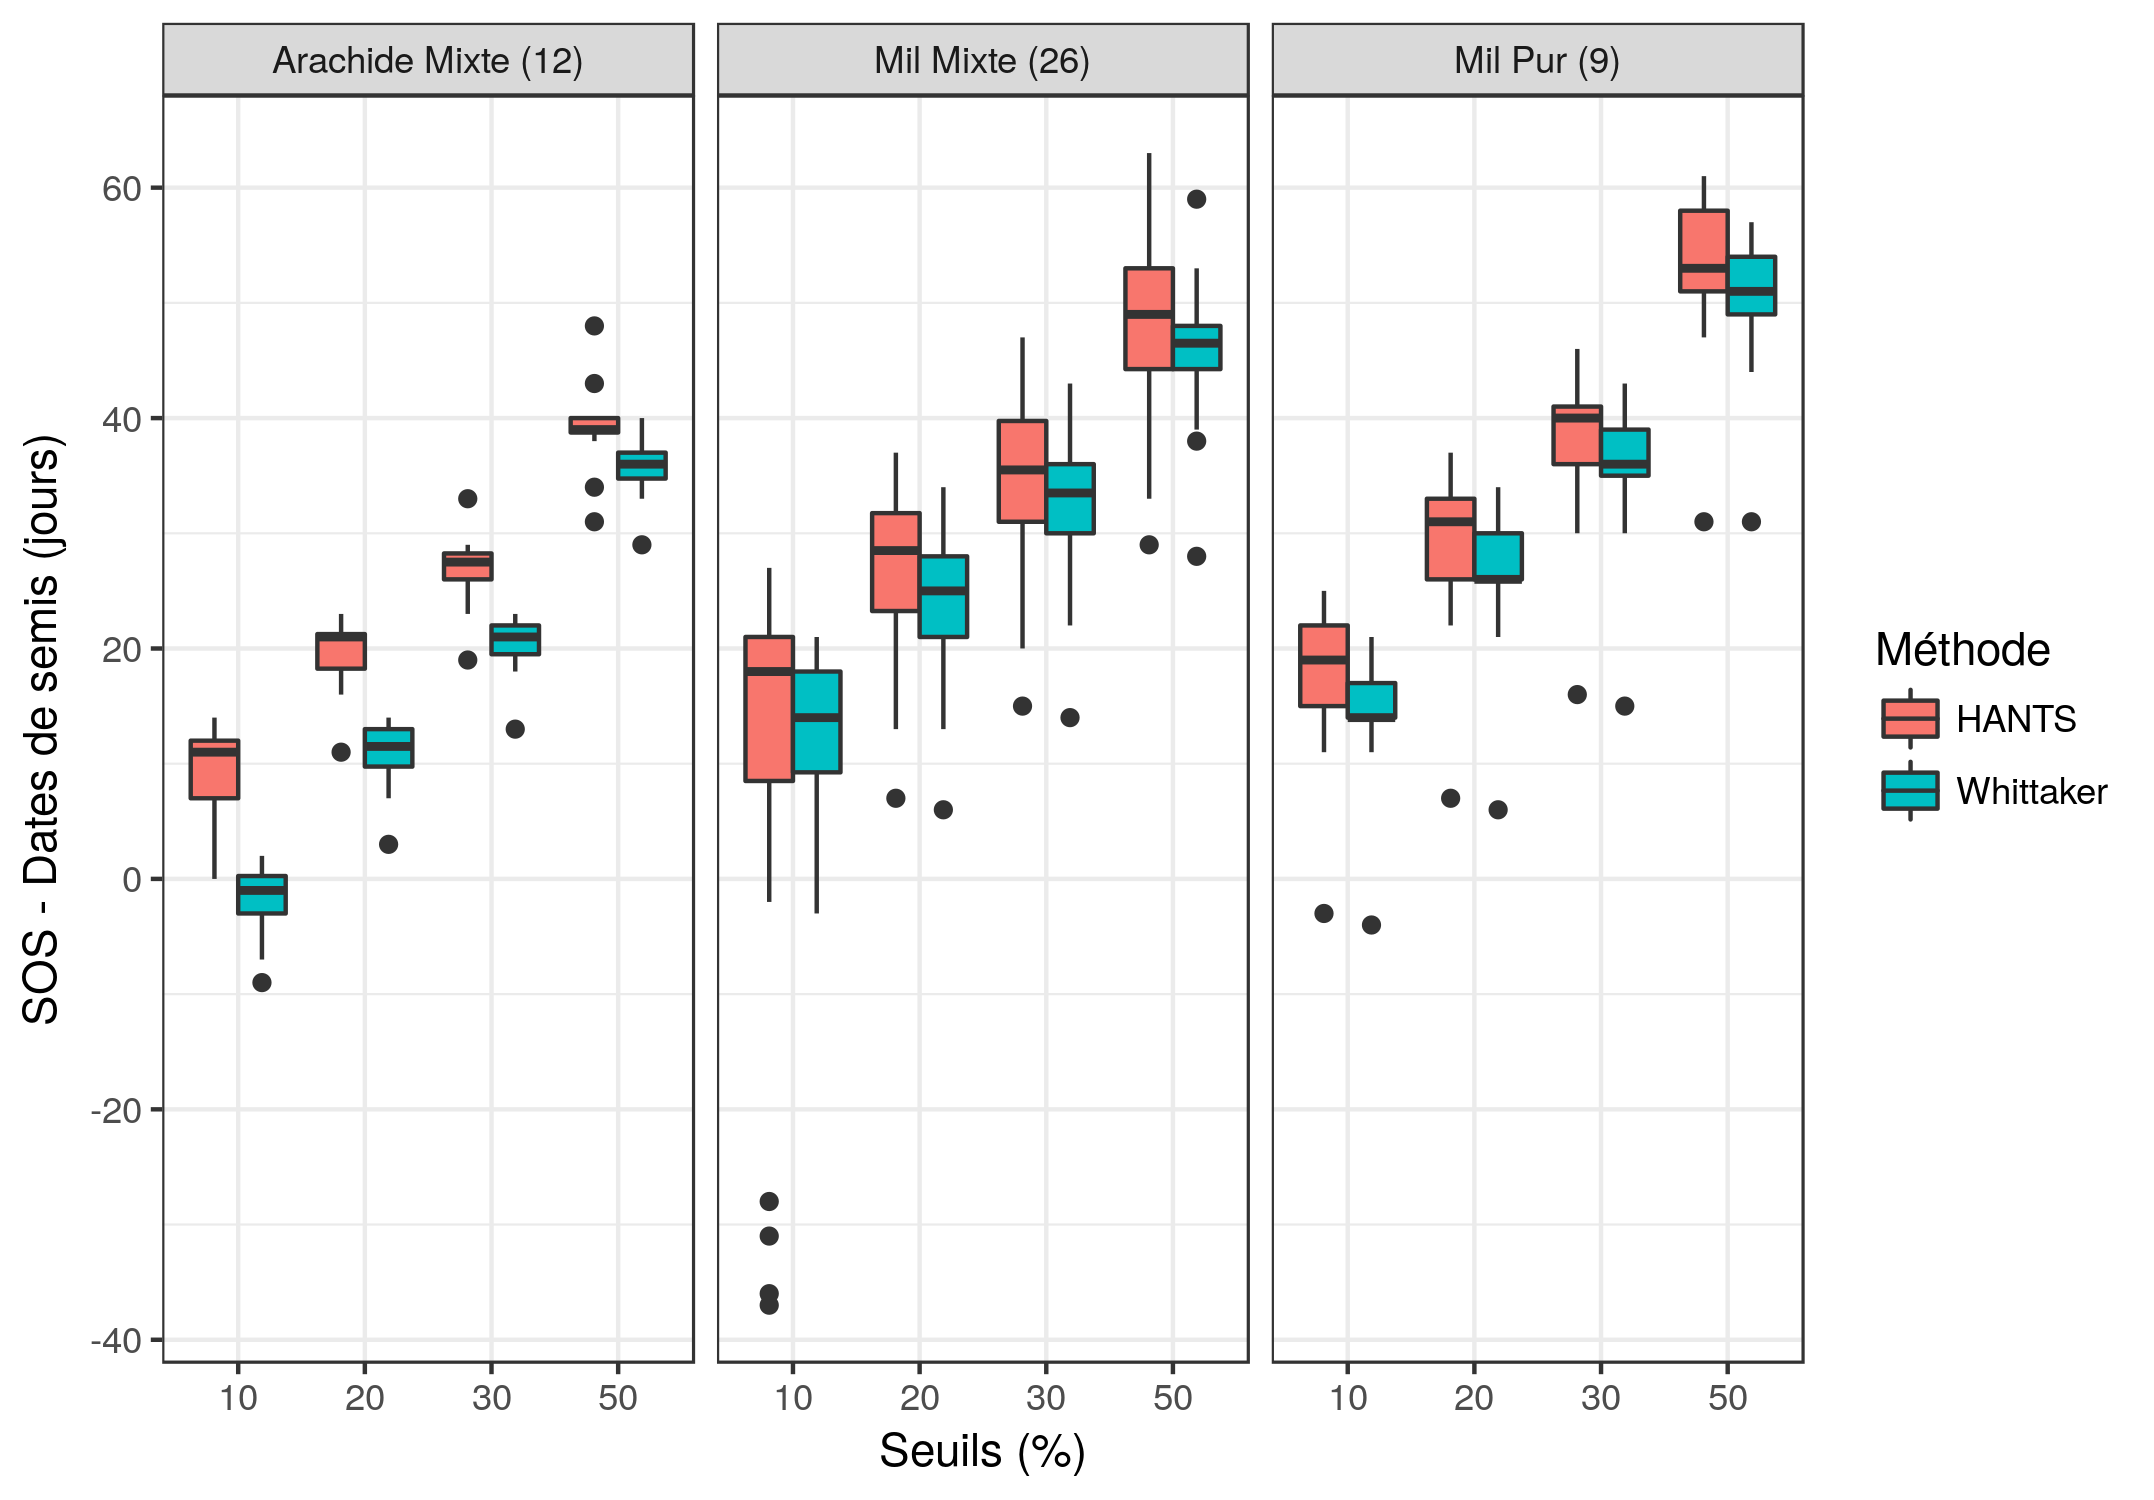
\includegraphics[scale=0.7]{resultats_discussions/SOS_Boxplot.png} 
 \end{center}
 \caption[Distribution des écarts entre SOS et dates de semis]{Boîtes à moustaches illustrant la distribution des écarts entre SOS estimés et dates de semis observées en fonction des systèmes de culture et des méthodes de lissage (\emph{Le nombre de parcelles est indiqué à la suite du système de culture})}
 \label{fig-sosboxplot}
\end{figure}

\newpage

La variation du RMSE en fonction du seuil d’extraction quelque soit le système de culture ou la méthode de lissage pris en compte rejoint l’analyse sur la distribution des écarts. En effet, plus le seuil d’extraction croit et plus le RMSE entre SOS et
dates de semis est grand, ce dernier étant un indicateur d’écart. La variation du CV en fonction du seuil d’extraction révèle d’abord deux valeurs qui portent à interrogation : -179\% (pour un seuil de 10\% avec la méthode de Whittaker sur les parcelles d’arachide mixte) et 200\% (pour un seuil de 10\% avec HANTS sur les parcelles de mil
mixte). L’analyse de nos résultats a montré qu’il s’agissait en fait de cas où l’écart-type était supérieure à une moyenne très petite proche de 0 (négative et positive respectivement). Ceci indique que les SOS extraits dans ces cas sont précoces. Pour le reste, la valeur du coefficient de variation diminue quand le seuil d’extraction croît, système de culture et méthode de lissage confondus. Ceci peut s’expliquer par le fait que la moyenne des écarts entre SOS et dates de semis augmente à mesure que le seuil d’extraction s’accroit quand l’écart-type ou la variabilité entre les écarts n’est pas très
différente. Finalement, il apparait que les seuils les plus adaptés sont celui de 20\% avec la méthode de Whittaker pour les parcelles d’arachide mixte, estimant les SOS avec un RMSE légèrement supérieur à 10 jours et ceux de de 10\% avec la méthode de Whittaker pour les parcelles de mil pur et de mil mixte, estimant les SOS avec des
RMSE de 15 jours.

\begin{figure}[htbp]
 \begin{center}
  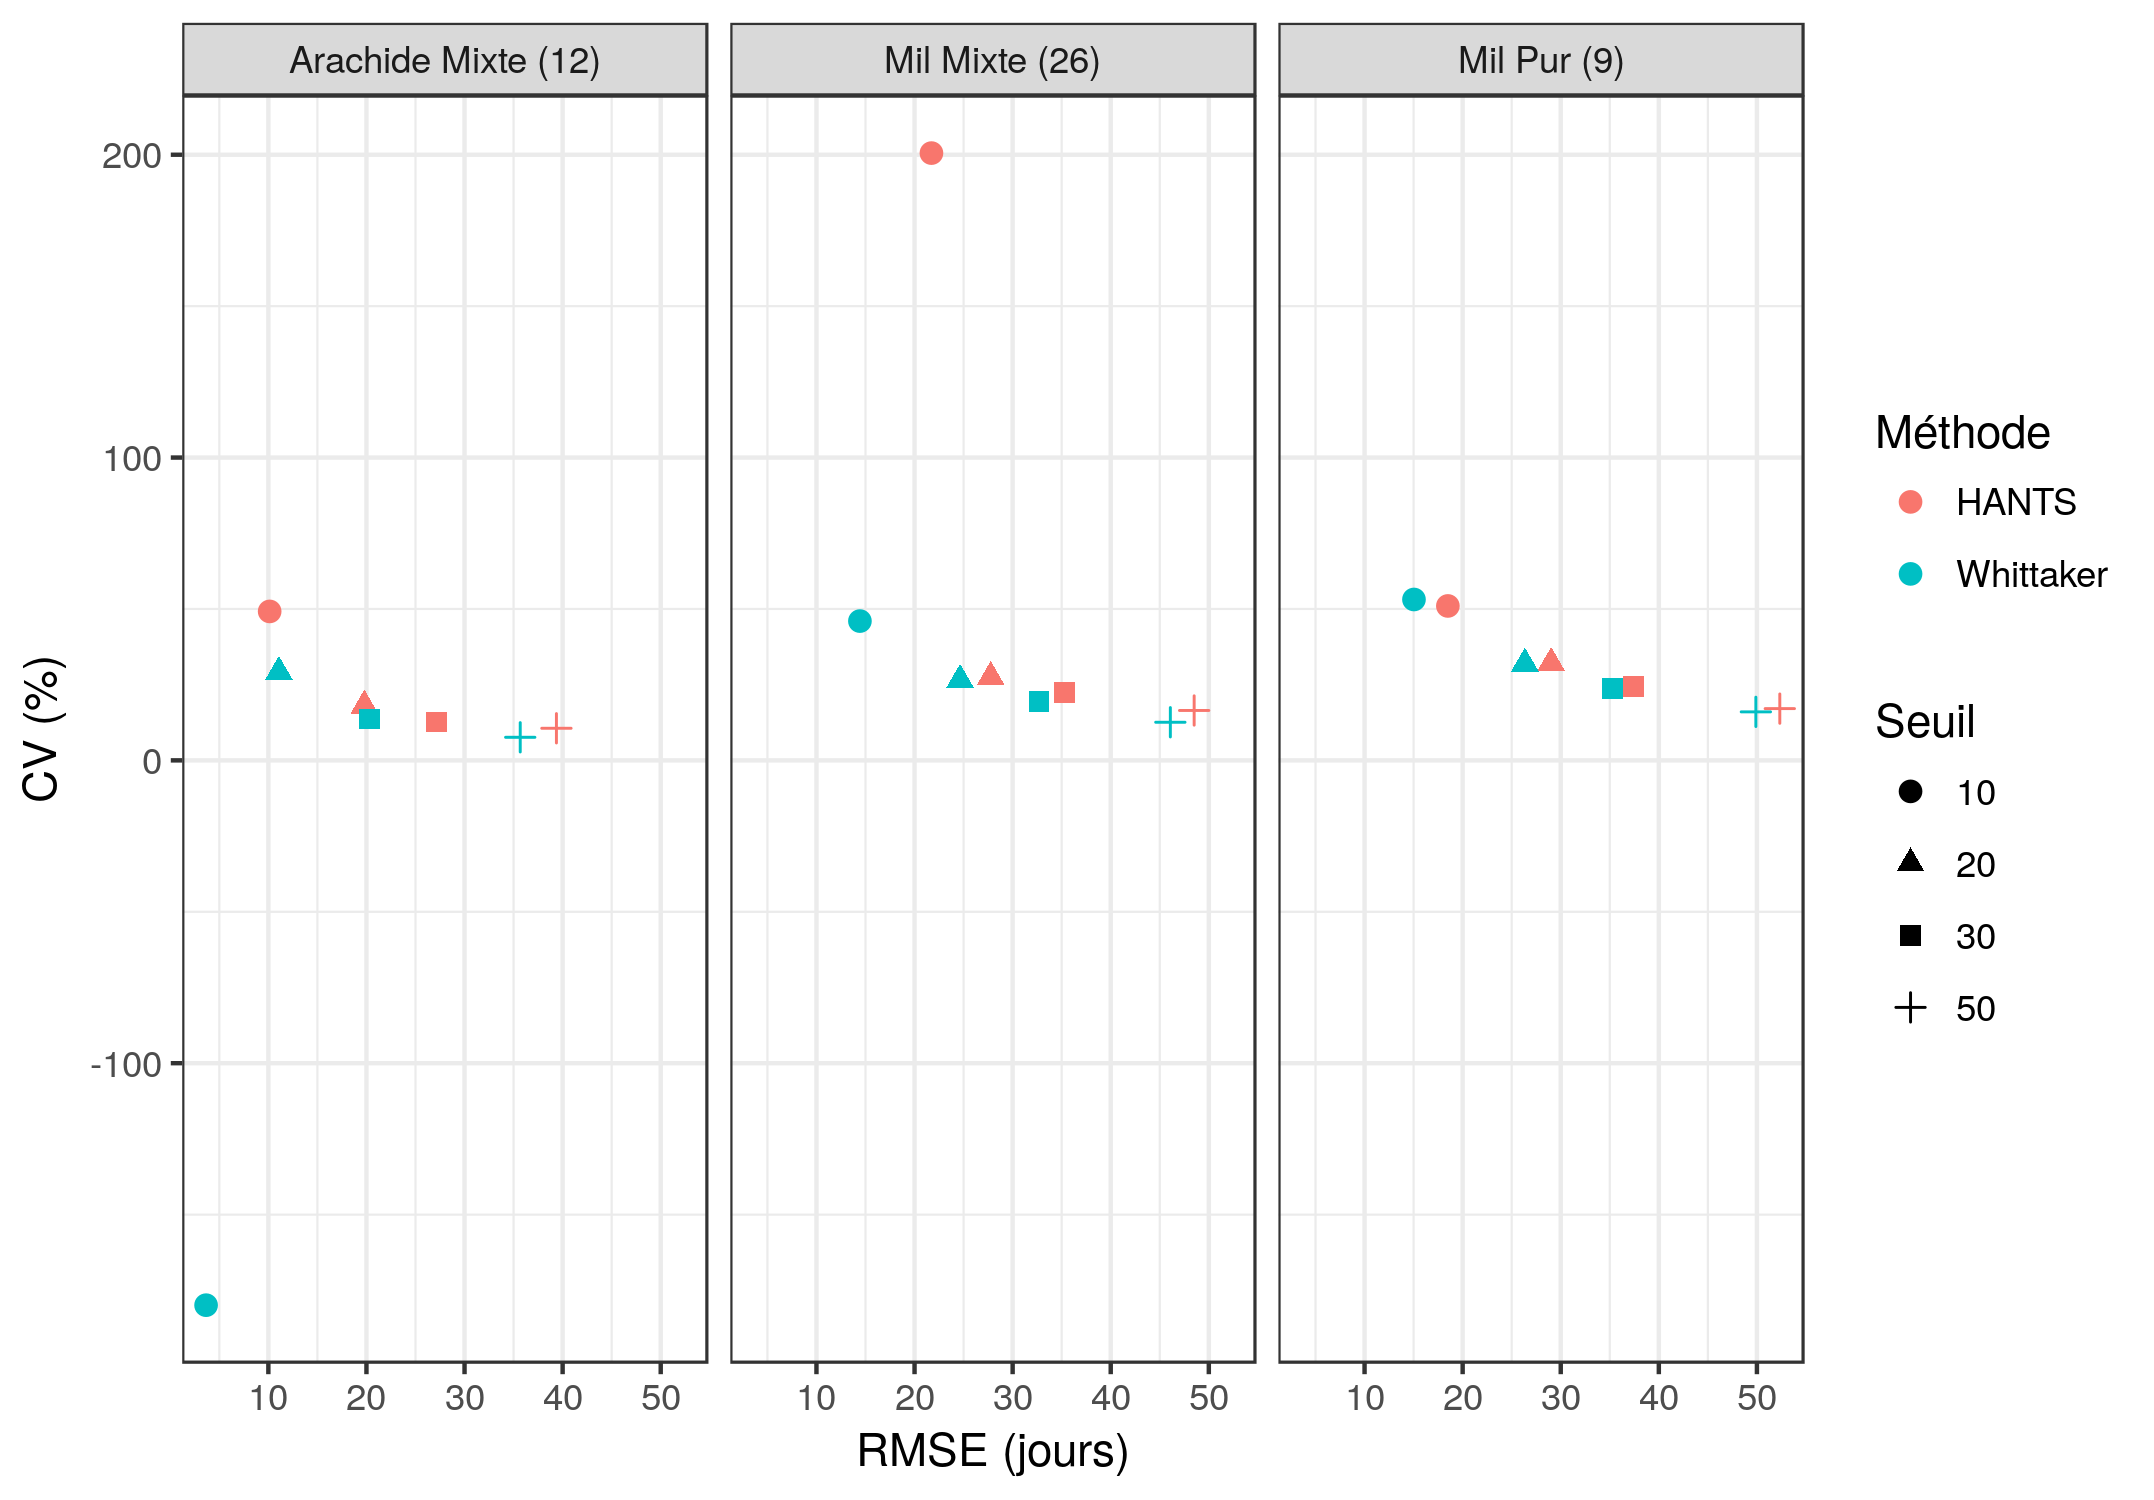
\includegraphics[scale=0.7]{resultats_discussions/SOS_RMSE_vs_CV.png} 
 \end{center}
 \caption[SOS -- RMSE vs CV]{Représentation du RMSE entre dates de semis et SOS estimés en fonction du coefficient de variation de leurs écarts par système de culture et méthode de lissage}
 \label{fig-sos-rmse-cv}
\end{figure}

\newpage

\paragraph{EOS}
Comme pour les SOS, nous avons représenté la distribution des écarts mais cette fois ci entre les dates de récoltes observées et les EOS extraits par système de culture et méthode de lissage (\Cref{fig-eosboxplot}). Les parcelles d’arachide mixte montrent légèrement moins de variabilité entre les écarts que les parcelles de mil mixte et de
mil pur. La plage des écarts obtenus avec les EOS estimés par HANTS est légèrement inférieure à celle des écarts obtenus avec les EOS extraits par la méthode de Whittaker notamment pour les parcelles d’arachide et de mil mixtes tous les seuils compris. En ce qui concerne la variation des seuils, nous avons des tendances différentes pour les parcelles d’arachide et de mil. Certes, plus on augmente les seuils d’extraction du EOS et plus les dates de fin de saison estimées se rapprochent des dates de récoltes mais cette précocité des EOS n’est pas obtenue au même moment pour les deux types de cultures. Ainsi, le seuil de 60\% extrait des EOS déjà trop précoces pour les parcelles d’arachide (médiane des écarts autour de 0 pour les 2 méthodes de lissage) tandis
que les EOS extraits pour les parcelles de mil avec un seuil de 80\% ont au moins 10 jours d’écart avec les dates de récoltes. Le seuil le plus adapté pour chaque système de culture doit déterminer les EOS en minimisant les écarts par rapport aux dates de récoltes et en réduisant au mieux la variabilité de ces écarts puisqu’en fin de compte les périodes de forte corrélation pour l’estimation des rendements qui viendra par la suite, ne doivent pas excéder les dates de récoltes.

\begin{figure}[htbp]
 \begin{center}
  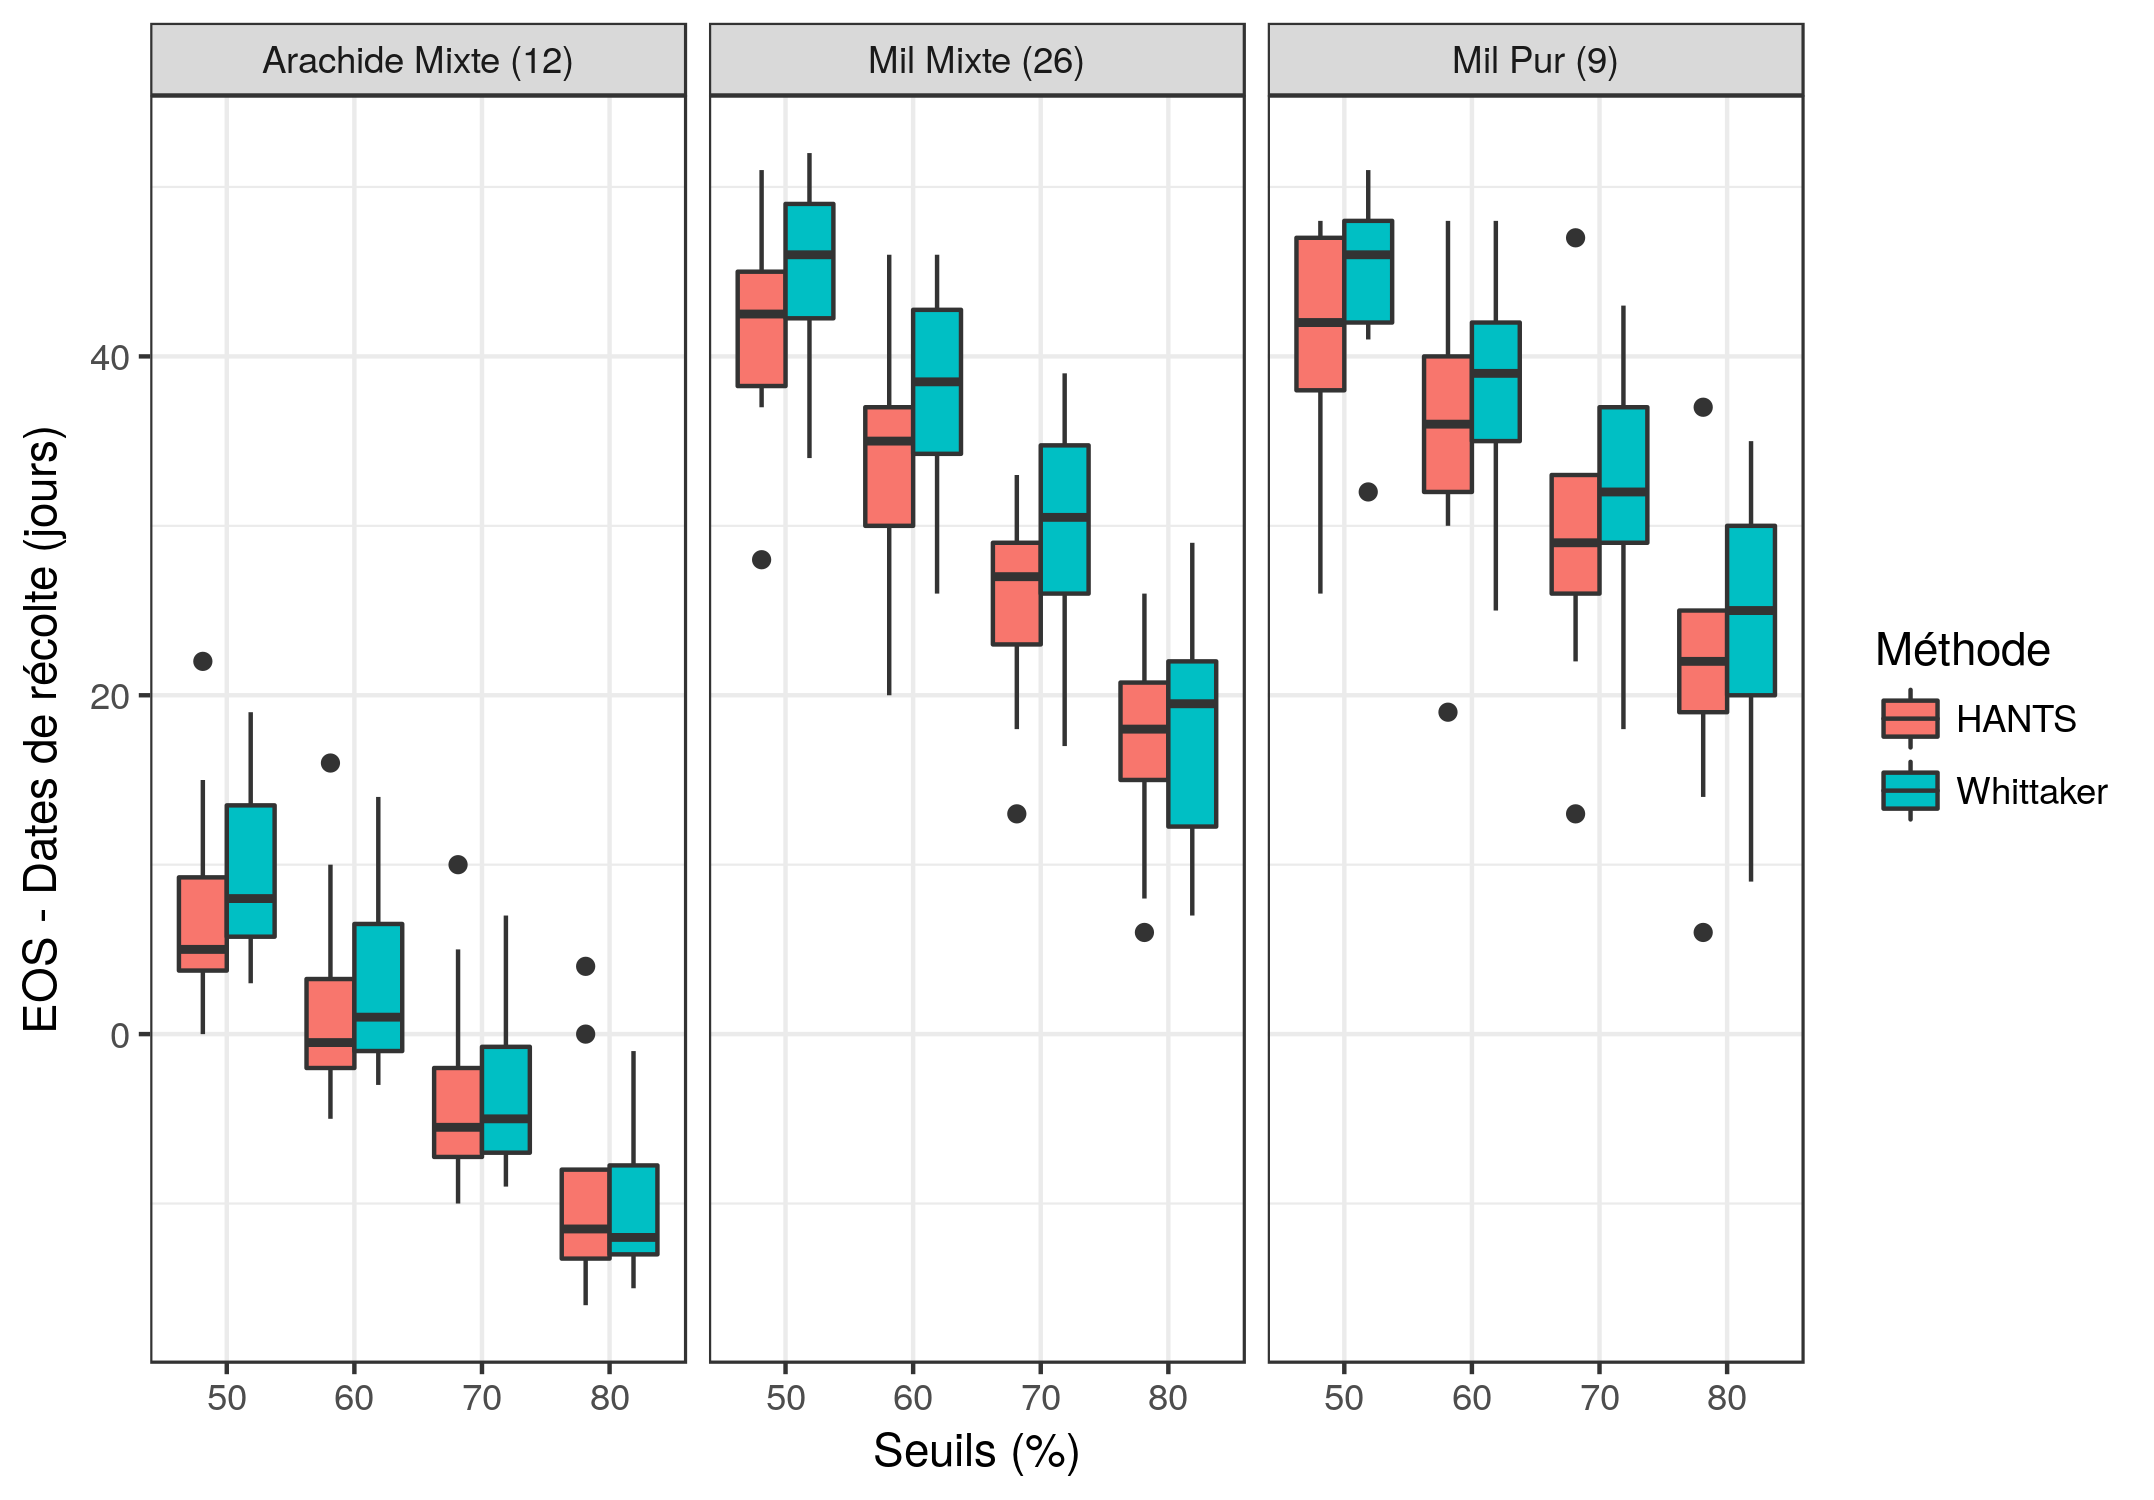
\includegraphics[scale=0.7]{resultats_discussions/EOS_Boxplot.png} 
 \end{center}
 \caption[Distribution des écarts entre EOS et dates de récoltes]{Boîtes à moustaches illustrant la distribution des écarts entre EOS estimés et dates de récoltes observées en fonction des systèmes de culture et des méthodes de lissage}
 \label{fig-eosboxplot}
\end{figure}

\newpage

Référons nous ensuite à la \cref{fig-eos-rmse-cv} où nous avons représenté la variation du RMSE en fonction du CV. Pour les parcelles d’arachide mixte, les RMSE les plus faibles sont obtenus avec les seuils de 60 et 70\% ce qui est normal car les écarts entre EOS et dates de récoltes à ces seuils sont faibles (proches de $0$). Par contre, leurs coefficients de variations très élevés rappellent le cas de dates précoces comme pour le SOS. Il apparait donc que le seuil le plus adapté pour l’extraction des EOS pour les parcelles d’arachide mixte est celui de 50\% car minimisant à la fois les écarts par rapport aux
dates de semis et leurs variabilités. Pour les parcelles de mil (pure et mixte confondus) par contre, le RMSE diminue à mesure que le seuil d’extraction augmente. Ainsi, les seuils de 80\% sont les plus adaptés car ils minimisent à la fois les écarts par rapport aux dates de semis et leur variabilité. En ce qui concerne la méthode de lissage
associée aux seuils choisis, celle de Whittaker est plus appropriée pour 2 raisons. La première raison se trouve dans l’estimation des SOS qui d’un point de vue agronomique est plus déterminante pour l’estimation des rendements finaux que celle des EOS et la méthode de Whittaker a été plus performante que HANTS sur ce point. L’autre raison se trouve dans le fait de garder un seul type de profil temporel pour
l’estimation des rendements en éliminant les profils lissés par HANTS et tout compte fait, les EOS obtenus avec les 2 méthodes de lissage ne sont pas aussi différents que les SOS estimés où il y’a nettement une supériorité des performances de la méthode de Whittaker.

\begin{figure}[htbp]
 \begin{center}
  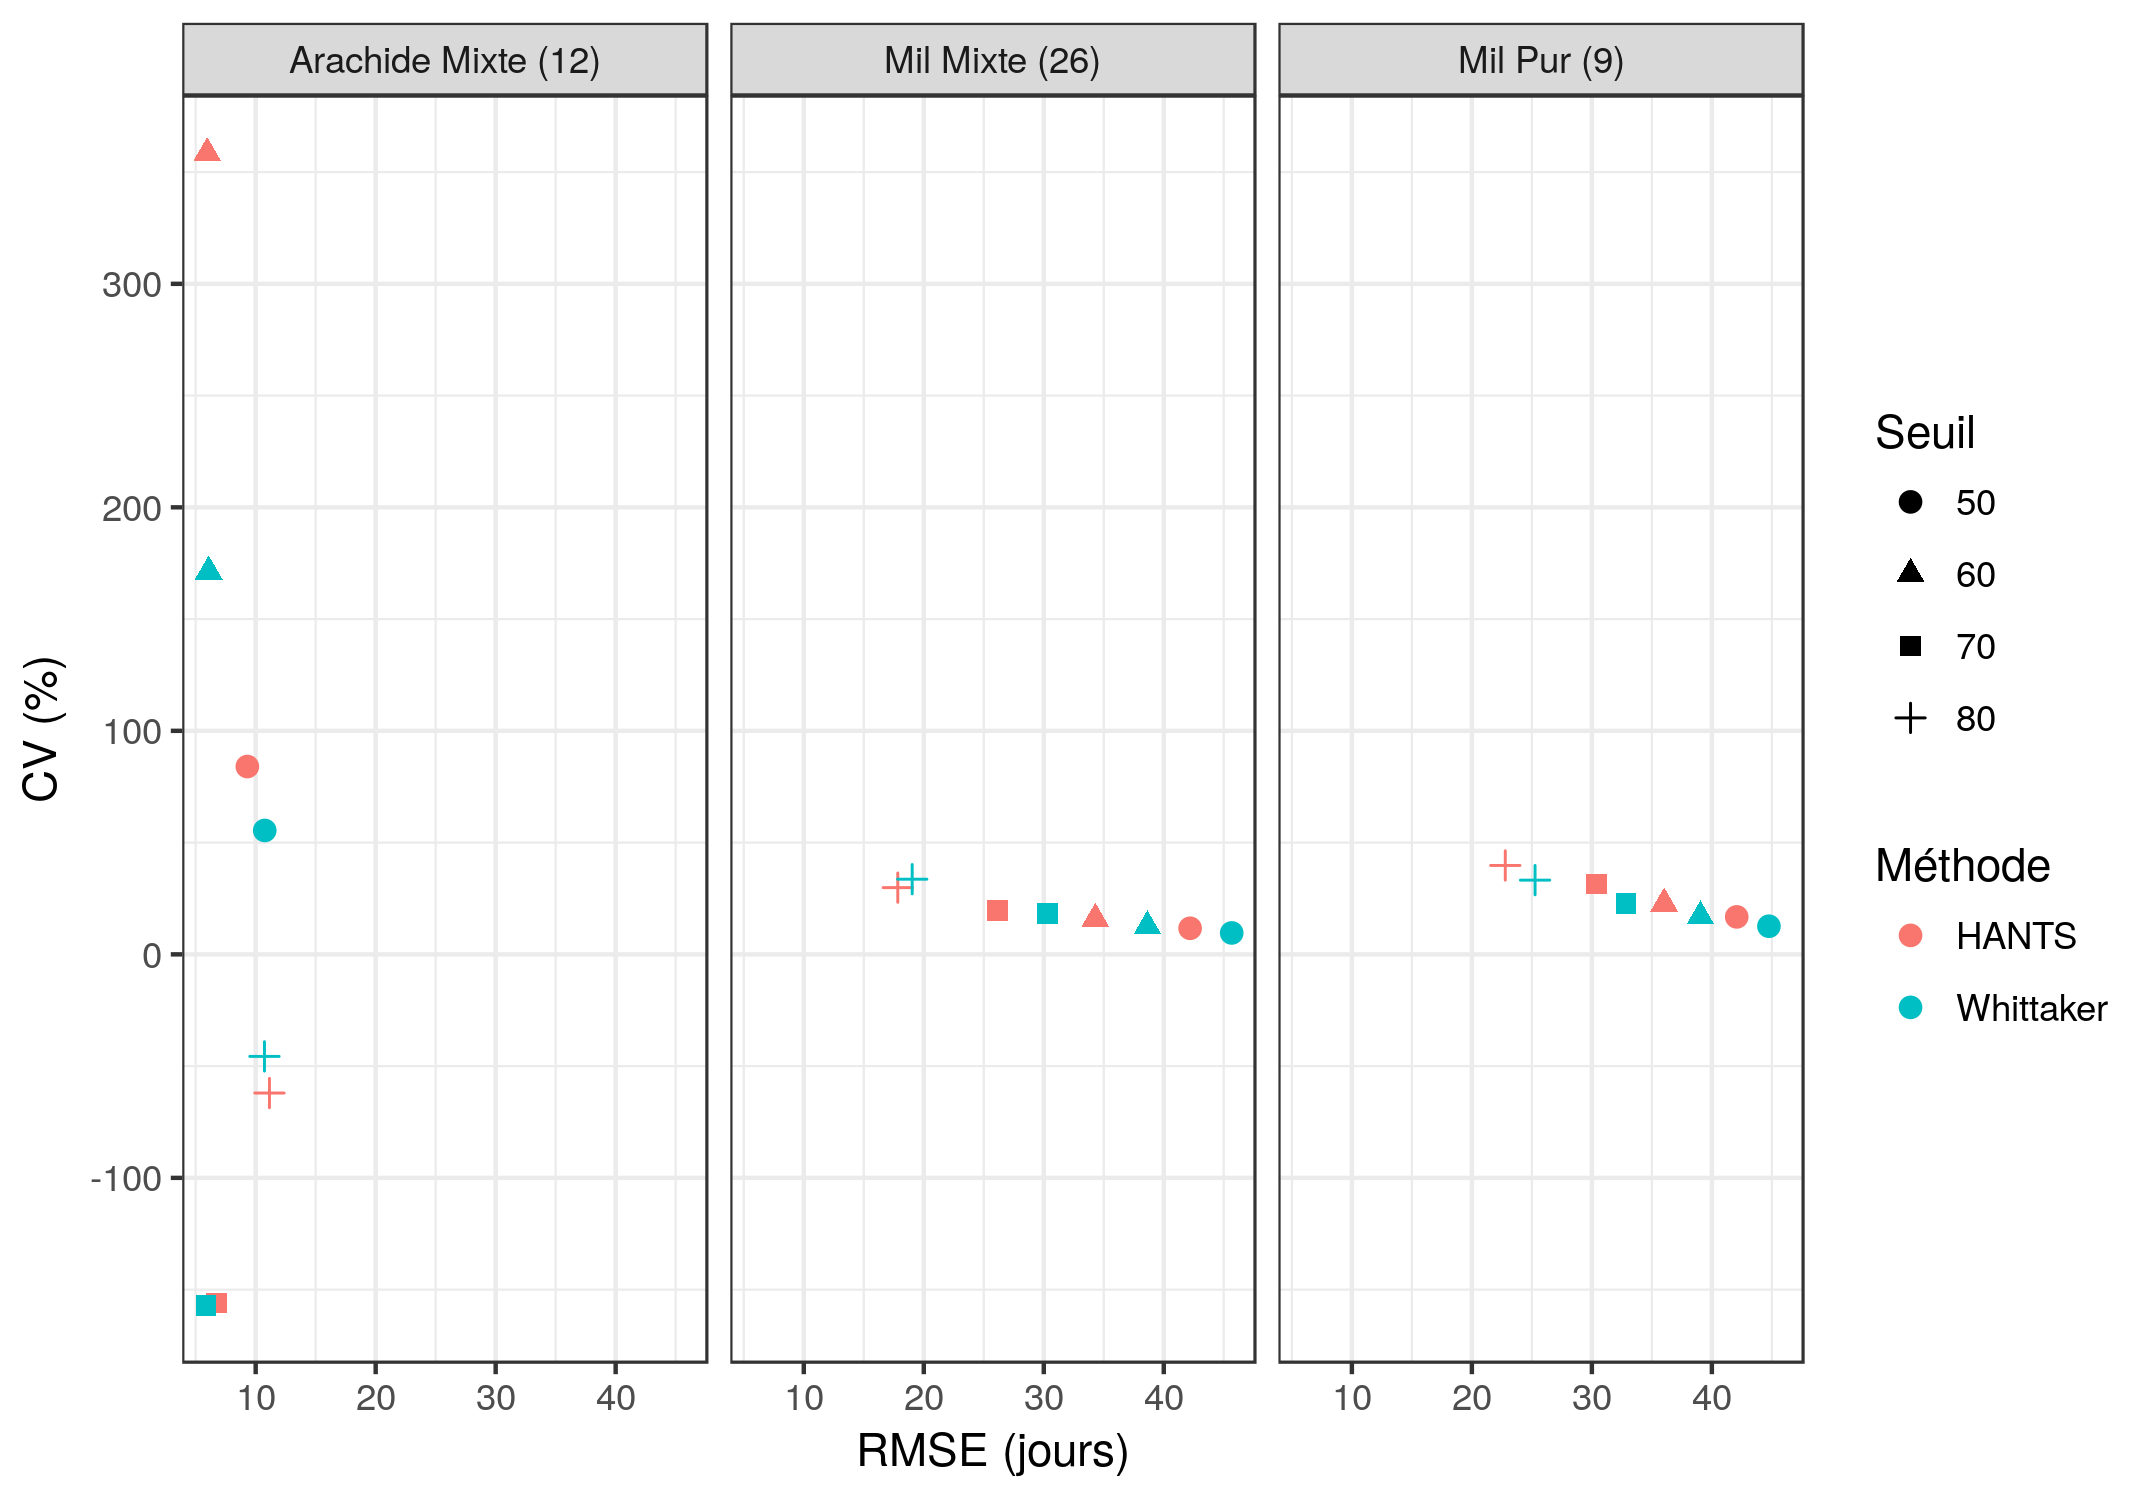
\includegraphics[scale=0.7]{resultats_discussions/EOS_RMSE_vs_CV.png} 
 \end{center}
 \caption[EOS -- RMSE vs CV]{Représentation du RMSE entre EOS estimés et dates de récoltes observées en fonction du coefficient de variation de leurs écarts par système de culture et méthode de lissage}
 \label{fig-eos-rmse-cv}
\end{figure}

\newpage 

Nous avons repris la même analyse sur l’estimation des SOS et des EOS en excluant les jeux de données de parcelles provenant du projet ANR-CERAO sans que les résultats présentés en \cref{annexe-c} soient significativement différents de ceux ci. La spatialisation des SOS et EOS avec les seuils adoptés est également présentée en \cref{annexe-d}.

\subsection{Estimation des biomasses et rendements}

Nous avons calibré 2 modèles de régression linéaire par type de culture pour estimer respectivement les biomasses et rendements observés. Afin de déterminer les meilleures variables explicatives pour chaque modèle, nous avons procédé en 2 étapes. Premièrement, nous avons cumulé les valeurs de NDVI et GDVI respectivement puis réalisé une régression linéaire à partir de chaque cumul effectué pour expliquer les biomasses et rendements. Nous avons ensuite aussi cherché les interactions possibles entre les métriques phénologiques calculées et les meilleures périodes d’intégration des indices, pouvant expliquer les biomasses et rendements observés. Au final, les variables explicatives retenues pour calibrer les modèles sont celles avec lesquelles nous avons obtenu les meilleures estimations de biomasses végétatives et rendements grain ou gousse, à condition que les régressions effectuées soient significatives.

\paragraph{Biomasses végétatives} 

Les résultats des régressions effectuées entre les biomasses
et les cumuls de NDVI et GDVI sont illustrés respectivement par les \cref{fig-cum-biom-ndvi,fig-cum-biom-gdvi}. Globalement, les cumuls de NDVI et de GDVI sont plus fortement corrélés à la biomasse de l’arachide qu’à celle du mil. Les cumuls de NDVI présentent de plus grandes périodes de fortes corrélations avec la biomasse de l’arachide que les cumuls de GDVI. Cependant, c’est le cumul des valeurs de GDVI entre 15 et 100 jours après le SOS ($CUM_{GDVI:15-100}$) qui explique mieux la biomasse de l’arachide avec un $R^{2}$ de $0,532$ et une p--value de $0,007$ contre un $R^{2}$ de $0,437$ et une p--value de $0,019$ pour le cumul des valeurs de NDVI sur un intervalle de 75 jours après le SOS ($CUM_{GDVI:0-75}$). Pour le mil par contre, ce sont les cumuls de GDVI qui sont plus corrélés à la biomasse. C’est le cumul des valeurs de GDVI entre 0 et 60 jours après le SOS ($CUM_{GDVI:0-60}$) qui explique le mieux la biomasse du mil avec un $R^{2}$ de $0,273$. La part de biomasse expliquée est certes faible mais reste significative avec une p--value de $0, 001$. Par la suite, les variables $CUM_{GDVI:15-100}$ et $CUM_{GDVI:0-60}$ renommées CUM afin d’uniformiser l’axe des $x$ sur la \cref{fig-inter-biom} ont respectivement été mises en interaction avec les métriques phénologiques calculées pour estimer la biomasse de l’arachide et du mil.

\begin{figure}[htbp]
 \begin{center}
  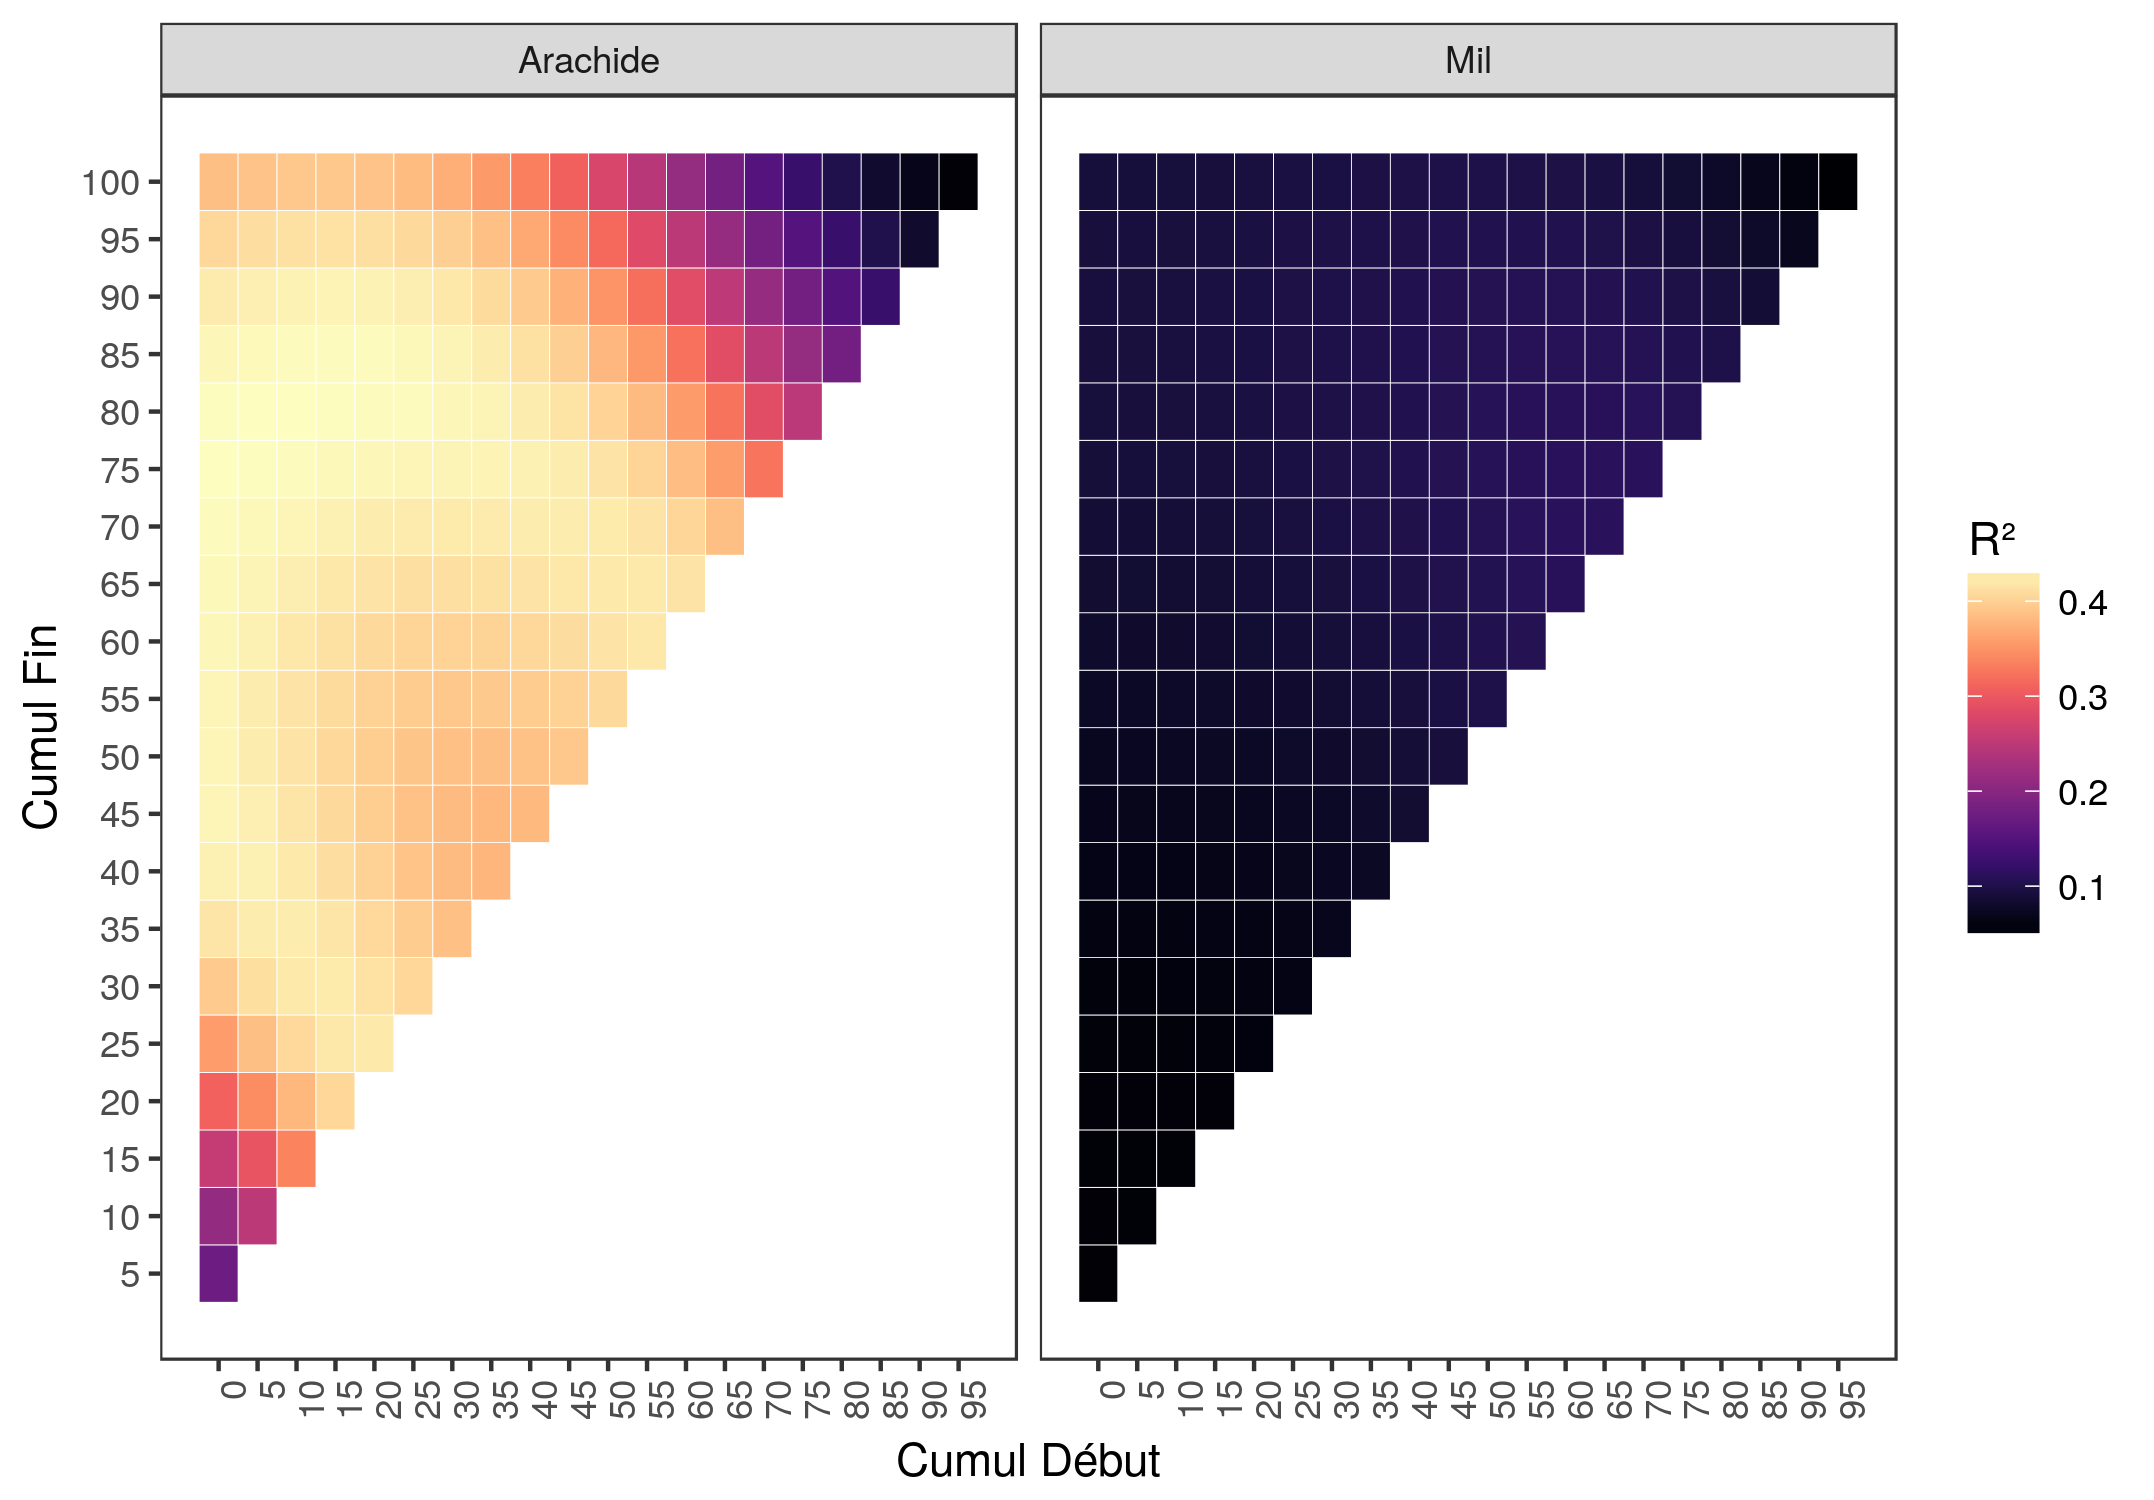
\includegraphics[scale=0.7]{resultats_discussions/Cum_Biom_NDVI.png} 
 \end{center}
 \caption[Régressions linéaires entre cumuls de NDVI et biomasses]{Résultats des régressions linéaires entre les cumuls de NDVI et les biomasses (\emph{l’axe x correspond au début du cumul et l’axe y à la fin du cumul ; le résultat de la régression entre les biomasses et les cumuls des valeurs de NDVI sur un intervalle de 5 jours après le SOS ($CUM_{NDVI:0-5}$) est donné par le croisement de la lecture de 0 sur l’axe des x et 5 sur l’axe des y})}
 \label{fig-cum-biom-ndvi}
\end{figure}

\begin{figure}[htbp]
 \begin{center}
  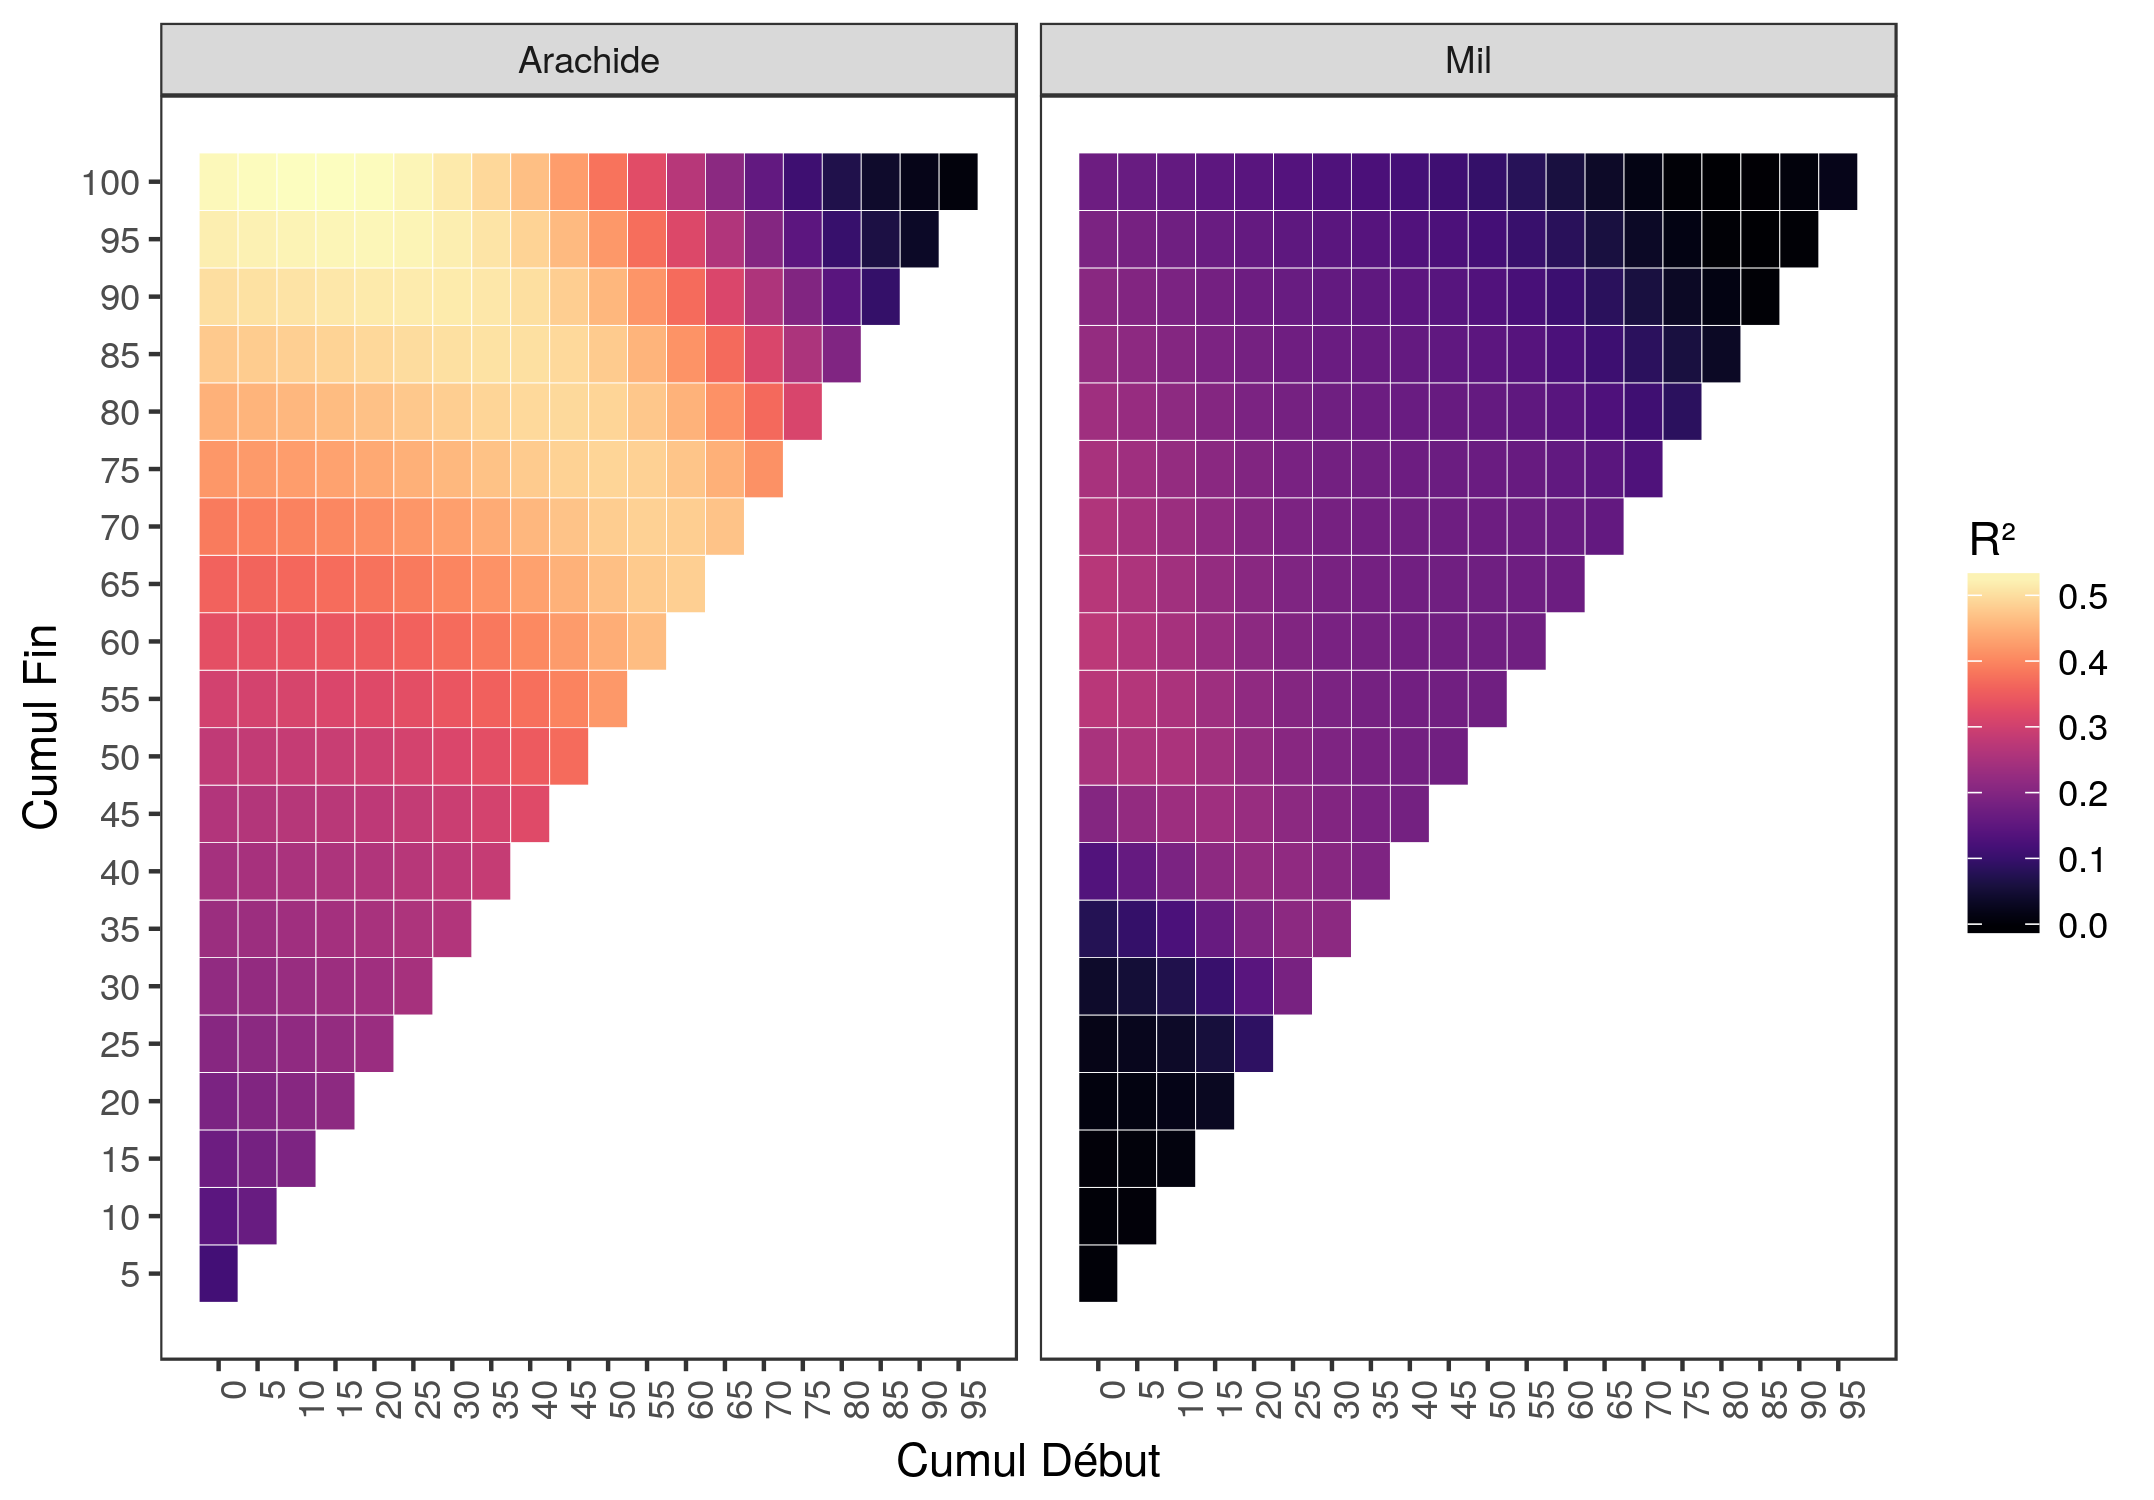
\includegraphics[scale=0.7]{resultats_discussions/Cum_Biom_GDVI.png} 
 \end{center}
 \caption[Régressions linéaires entre cumuls de GDVI et biomasses]{Résultats des régressions linéaires entre les cumuls de GDVI et les biomasses}
 \label{fig-cum-biom-gdvi}
\end{figure}

\begin{figure}[htbp]
 \begin{center}
  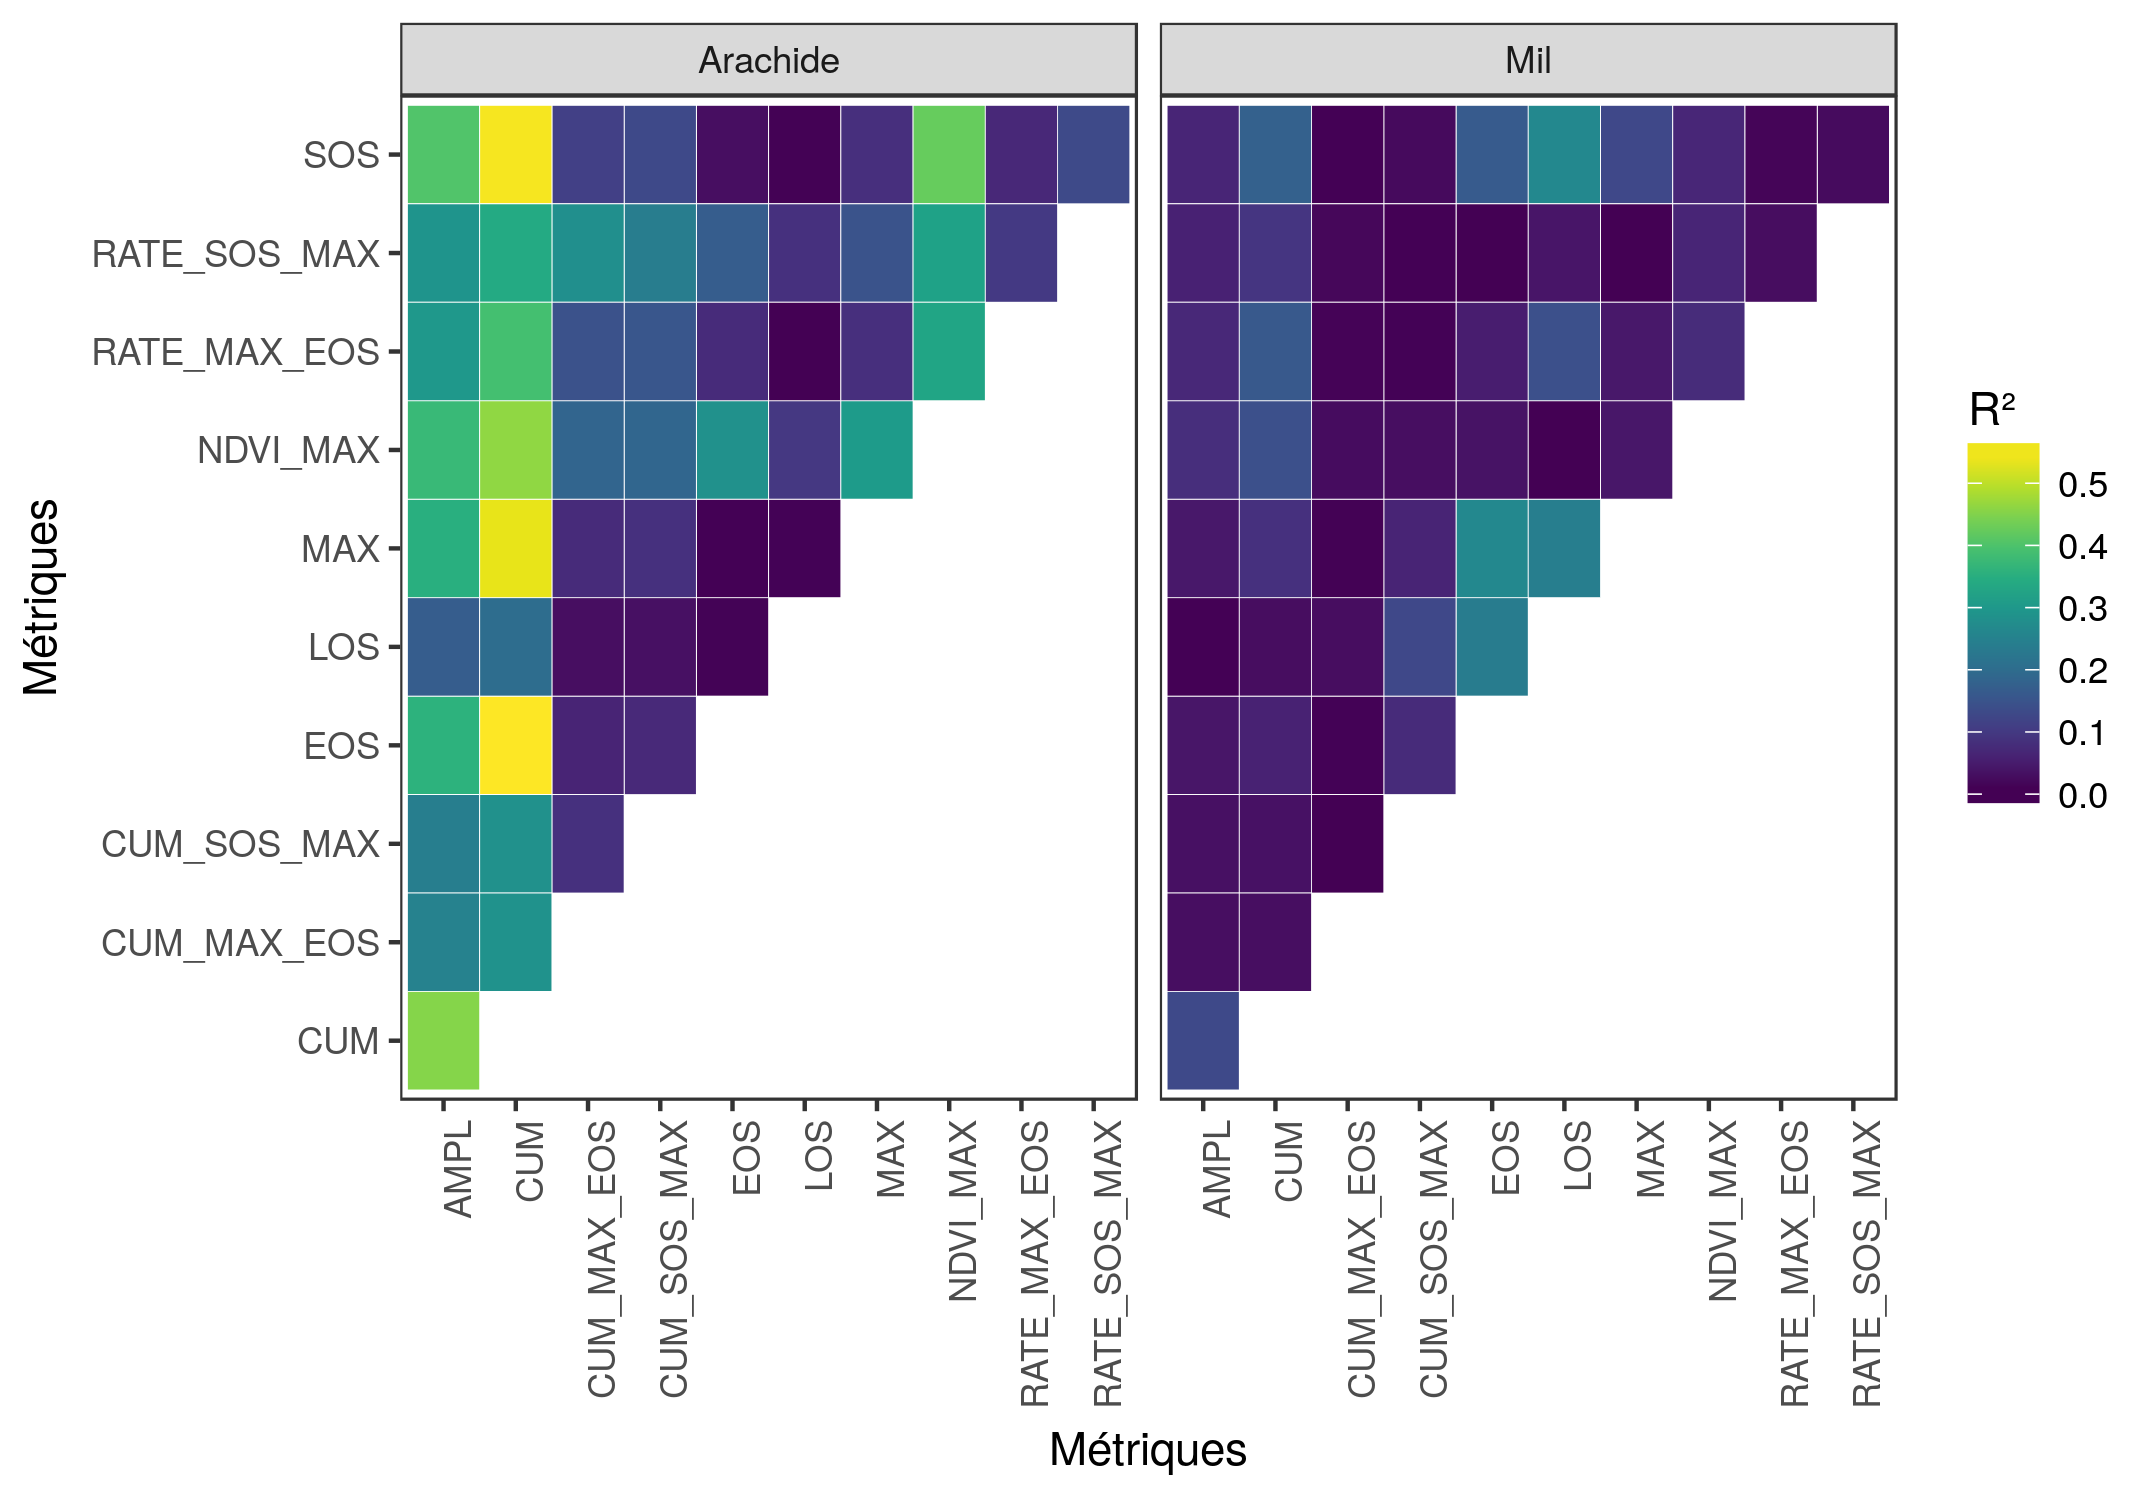
\includegraphics[scale=0.7]{resultats_discussions/Inter_Biom.png} 
 \end{center}
 \caption[Régressions linéaires entre interactions et biomasses]{Résultats des régressions linéaires entre les interactions de variables et les biomasses (\emph{l’axe des x donne le premier élément de l’interaction et l’axe des y le second ; le résultat de la régression linéaire entre l’interaction du SOS et du EOS ($SOS : EOS$) et les biomasses est donné par le croisement de la lecture de SOS sur l’axe des x et EOS sur l’axe des y})}
 \label{fig-inter-biom}
\end{figure}

Les résultats des régressions entre les interactions de variables et les biomasses de
l’arachide et du mil sont reportés sur la \cref{fig-inter-biom}. Les interactions des métriques
EOS, MAX et SOS avec la variable $CUM_{GDVI:15-100}$ sont celles qui ressortent pour
l’arachide et c’est l’interaction $EOS:CUM_{GDVI:15-100}$ qui explique le mieux la biomasse de l’arachide avec un $R^{2}$ de $0,562$ et une p--value de $0,005$. Pour le mil, c’est
l’interaction entre le MAX et le EOS qui explique mieux la biomasse avec un $R^{2}$
toujours faible de $0,263$ mais significatif avec une p--value de $0,002$. L’interaction
$EOS:CUM_{GDVI:15-100}$ explique mieux les biomasses de l’arachide tandis que celles
du mil sont plus corrélés avec la période d’intégration du GDVI sur un intervalle de
60 jours après le SOS. Au final, nous avons adopté les modèles de régression linéaire
avec les variables $EOS:CUM_{GDVI:15-100}$ et $CUM_{GDVI:0-60}$ respectivement pour l’es-
timation des biomasses de l’arachide et du mil (\Cref{fig-model-biom}).

\begin{figure}[htbp]
 \begin{center}
  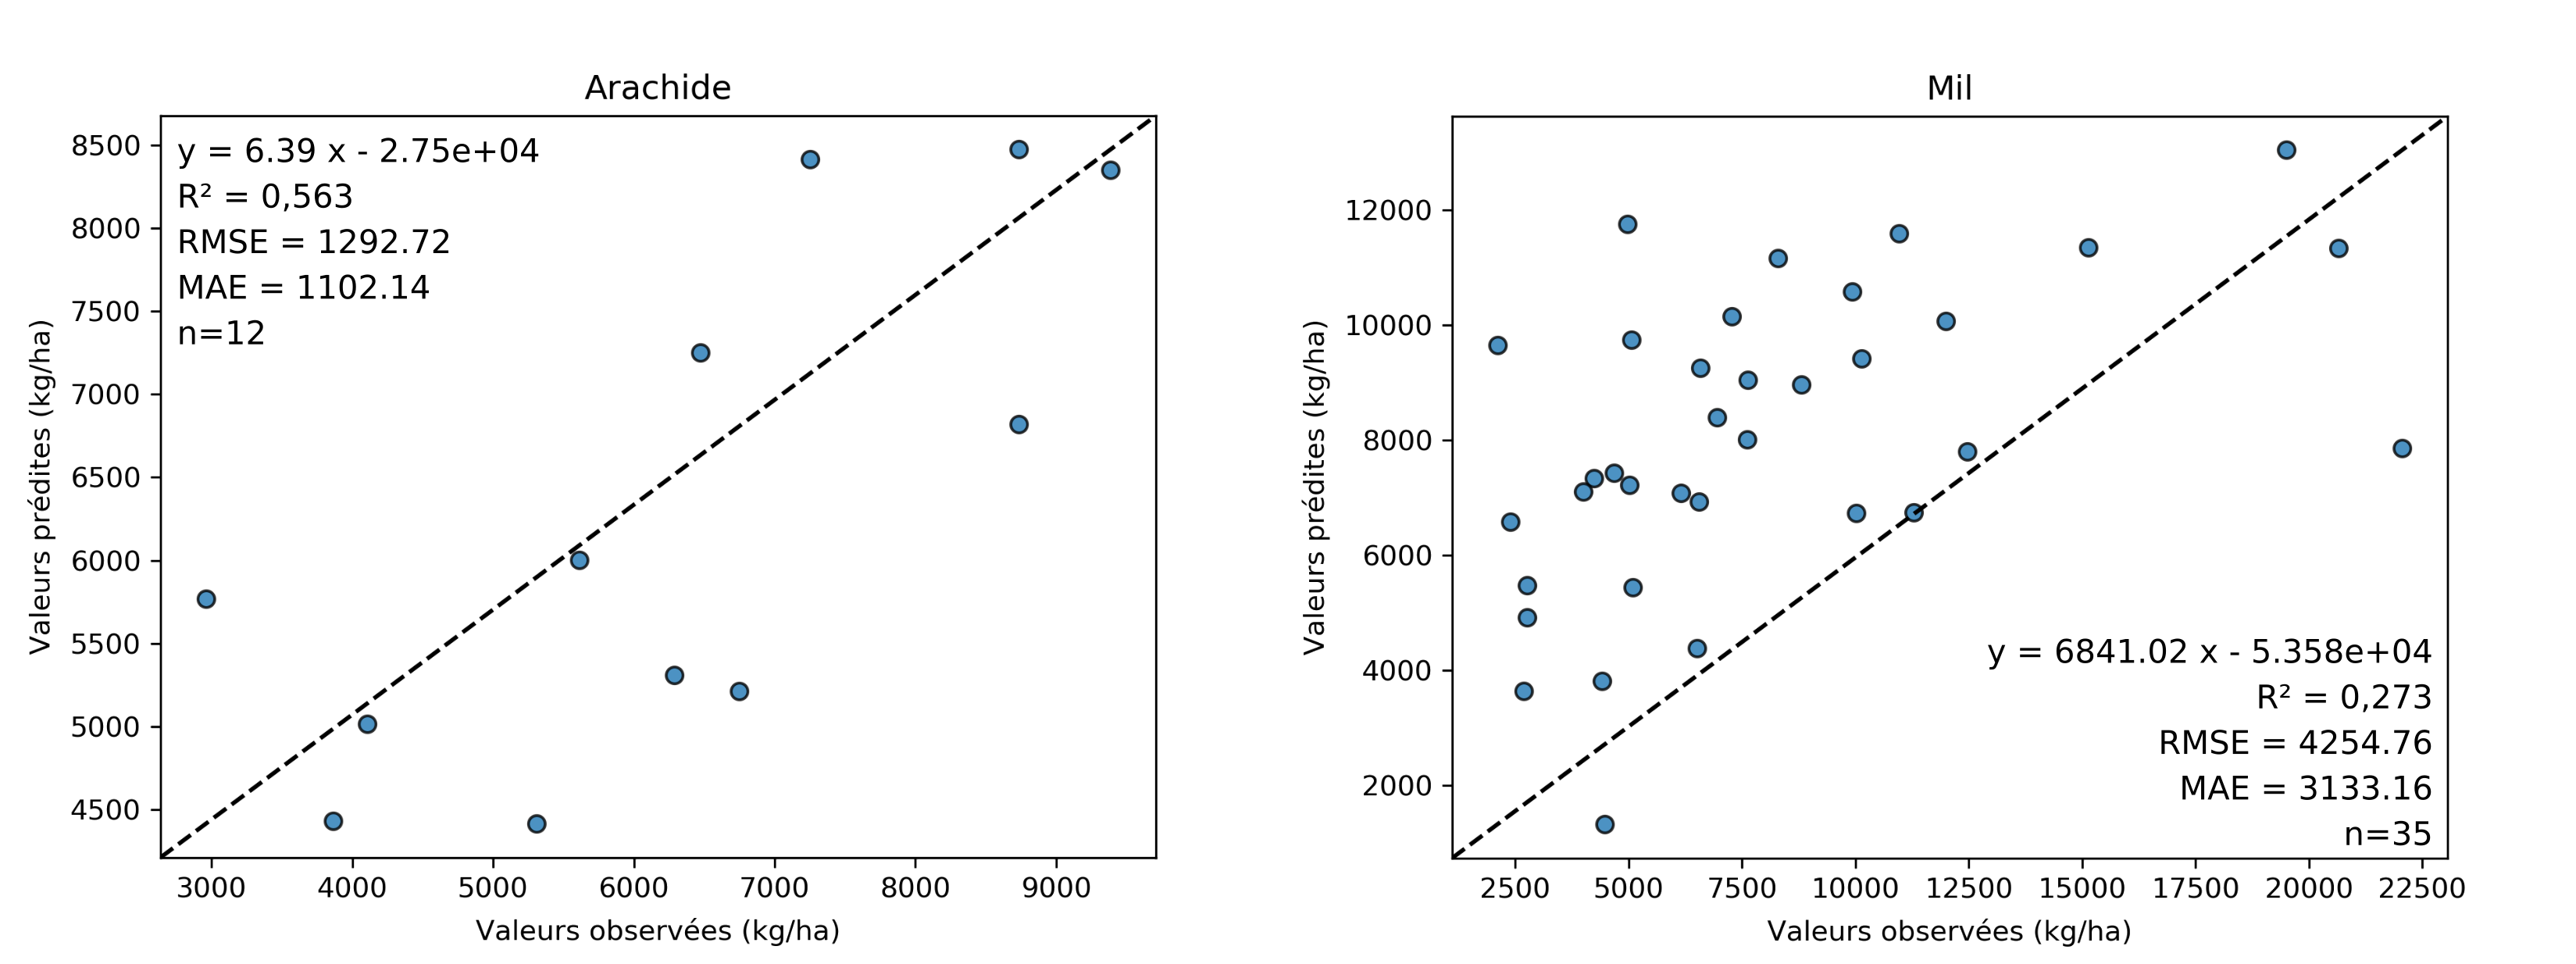
\includegraphics[scale=0.6]{resultats_discussions/Model_Biom.png} 
 \end{center}
 \caption[Modèles finaux pour l’estimation des biomasses]{Modèles finaux pour l’estimation des biomasses de l’arachide et du mil}
 \label{fig-model-biom}
\end{figure}

\paragraph{Rendements} 

Les résultats des régressions effectuées entre les rendements et les cumuls de NDVI et GDVI sont illustrés respectivement par les \cref{fig-cum-rdt-ndvi,fig-cum-rdt-gdvi}. Globalement, les cumuls de NDVI et de GDVI sont plus corrélés aux rendements du mil qu’à ceux de l’arachide. Toutes les périodes d’intégration du NDVI sont pratiquement corrélées avec les rendements du mil contre une majeure partie au milieu du cycle de développement du mil pour les périodes d’intégration du GDVI. Cependant, c’est le cumul des valeurs de GDVI entre 0 et 65 jours après le SOS ($CUM_{GDVI:0-65}$) qui explique mieux les rendements du mil avec un $R^{2}$ de $0,419$ et une p--value de $2,7\times10^{-5}$ contre un $R^{2}$ de $0, 316$ et une p--value de $4,33\times10^{-4}$ pour le cumul des valeurs de NDVI entre 60 et 65 jours après le SOS ($CUM_{NDVI:60-65}$). Pour l’arachide par contre, ce sont les cumuls de GDVI au tout début du cycle de développement qui sont plus corrélés aux rendements. C’est le cumul des valeurs de GDVI entre 15 et 20 jours après le SOS ($CUM_{GDVI:15-20}$) qui explique le mieux les rendements de l’arachide avec un $R^{2}$ de $0,363$ et une p--value de $0,038$. Par la suite, les variables $CUM_{GDVI:15-20}$ et $CUM_{GDVI:0-65}$ renommées CUM afin d’uniformiser l’axe des $x$ sur la \cref{fig-inter-rdt} ont respectivement été mis en interaction avec les métriques phénologiques calculées pour estimer les rendements gousses de l’arachide et grains du mil.

\begin{figure}[htbp]
 \begin{center}
  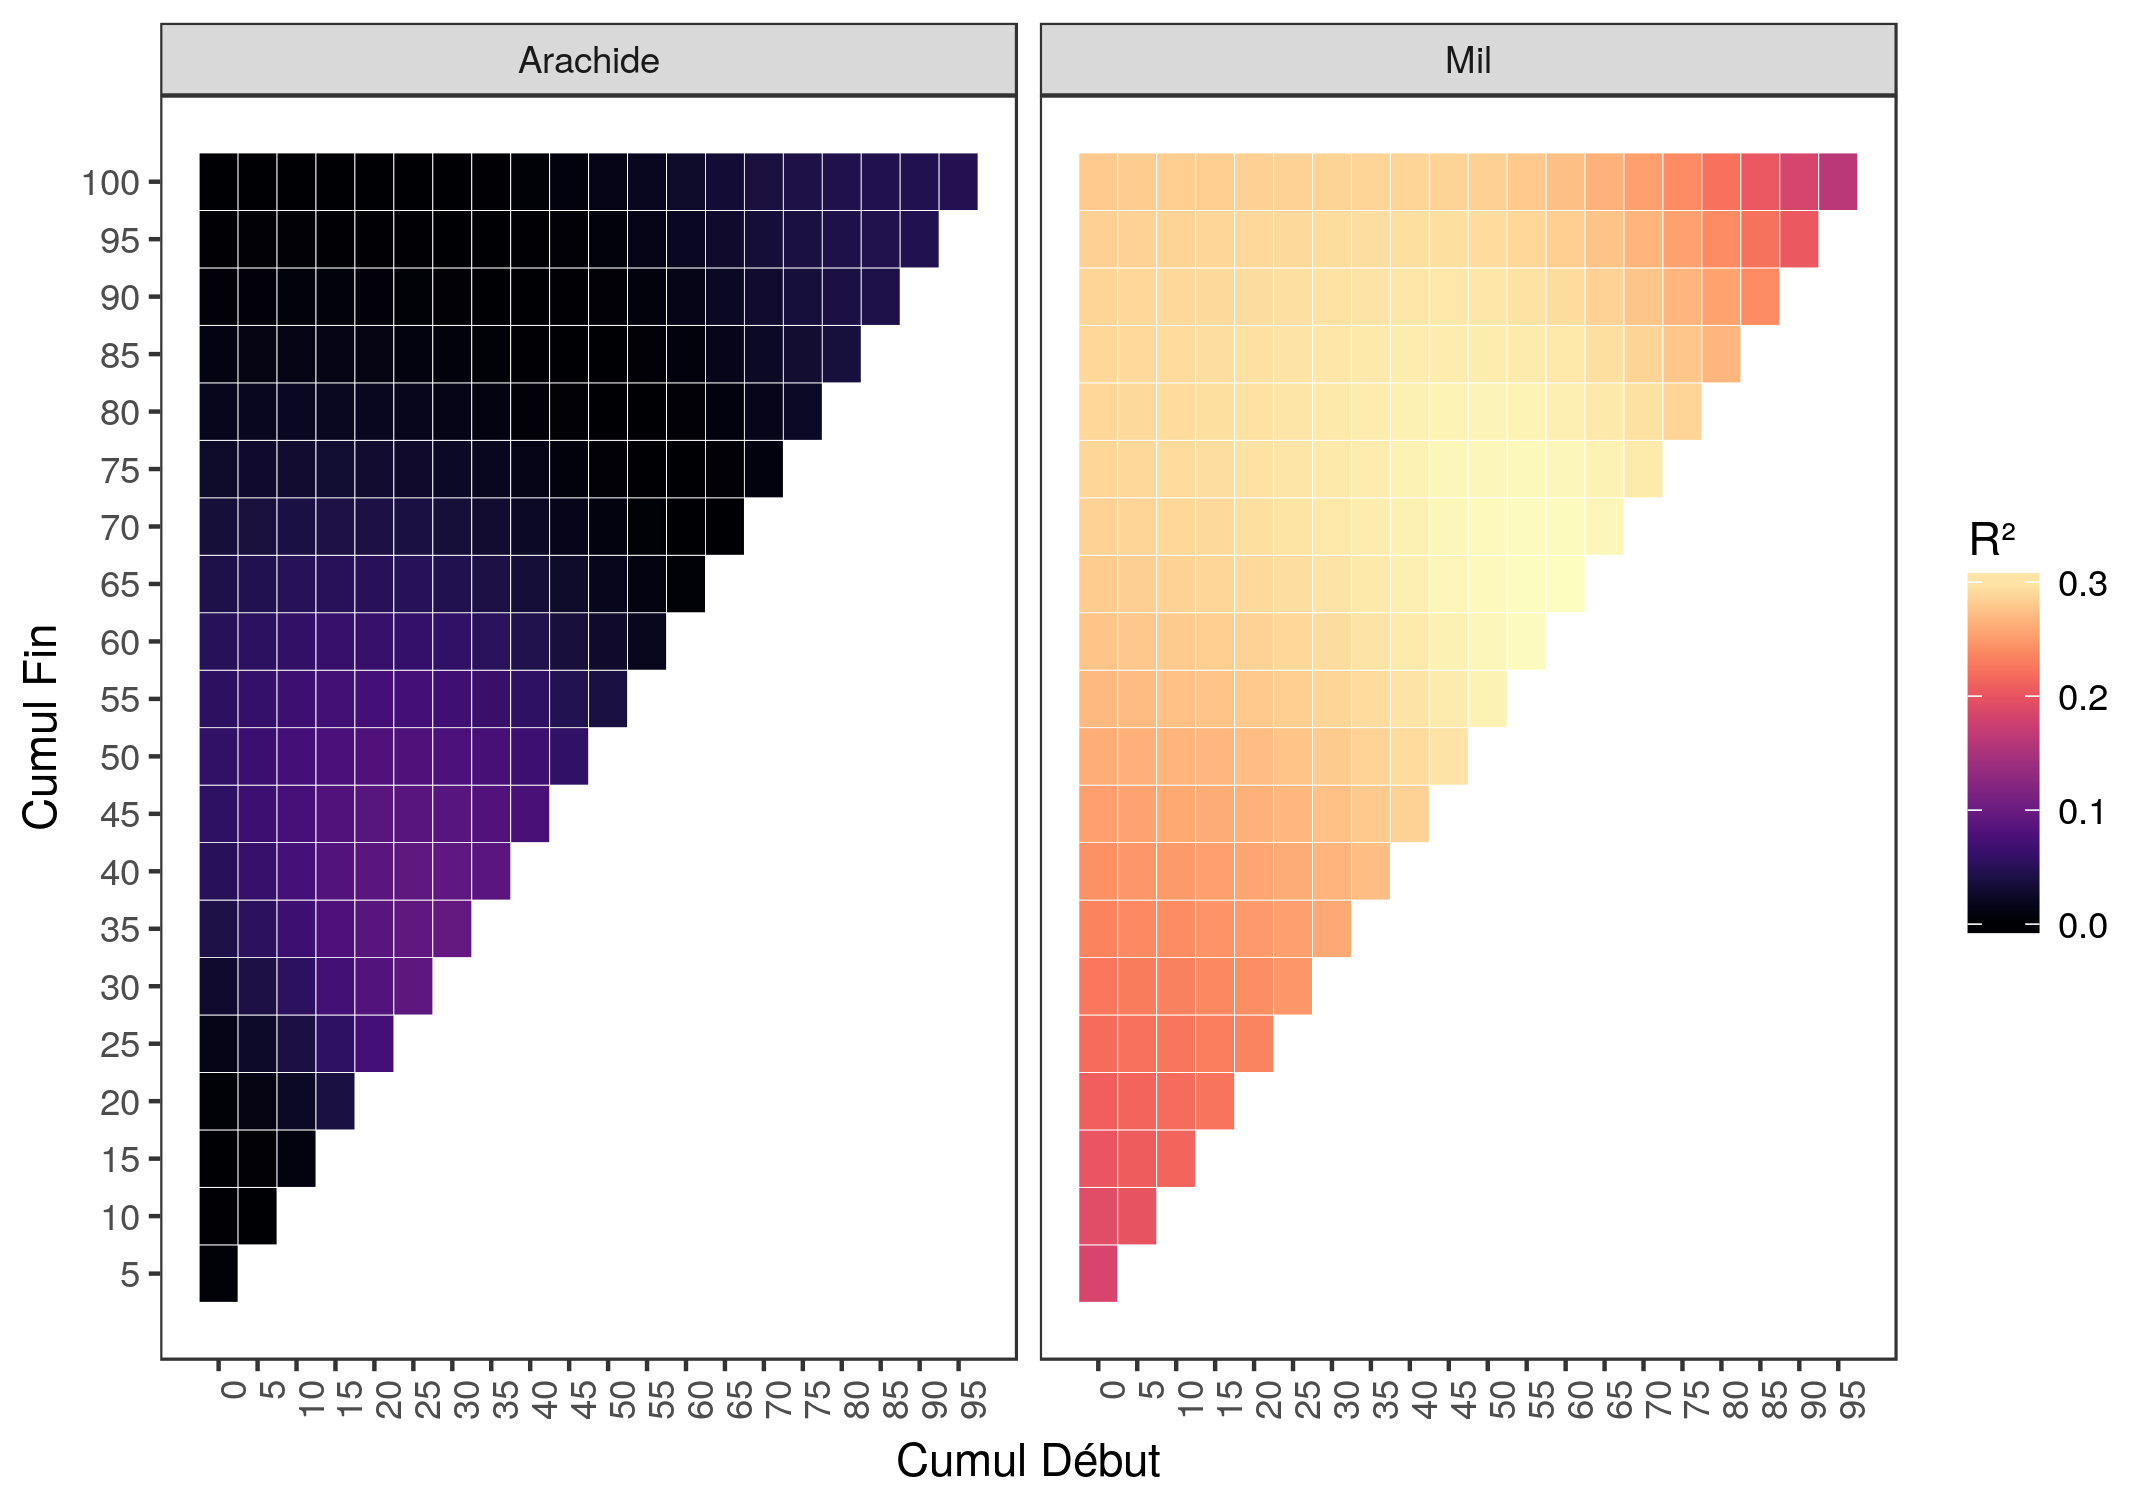
\includegraphics[scale=0.7]{resultats_discussions/Cum_Rdt_NDVI.png} 
 \end{center}
 \caption[Régressions linéaires entre cumuls de NDVI et rendements]{Résultats des régressions linéaires entre les cumuls de NDVI et les rendements (\emph{l’axe x correspond au début du cumul et l’axe y à la fin du cumul ; le résultat de la régression entre les rendements et les cumuls des valeurs de NDVI entre 5 et 10 jours après le SOS ($CUM_{NDVI:5-10}$) est donné par le croisement de la lecture de 5 sur l’axe des x et 10 sur l’axe des y})}
 \label{fig-cum-rdt-ndvi}
\end{figure}

\begin{figure}[htbp]
 \begin{center}
  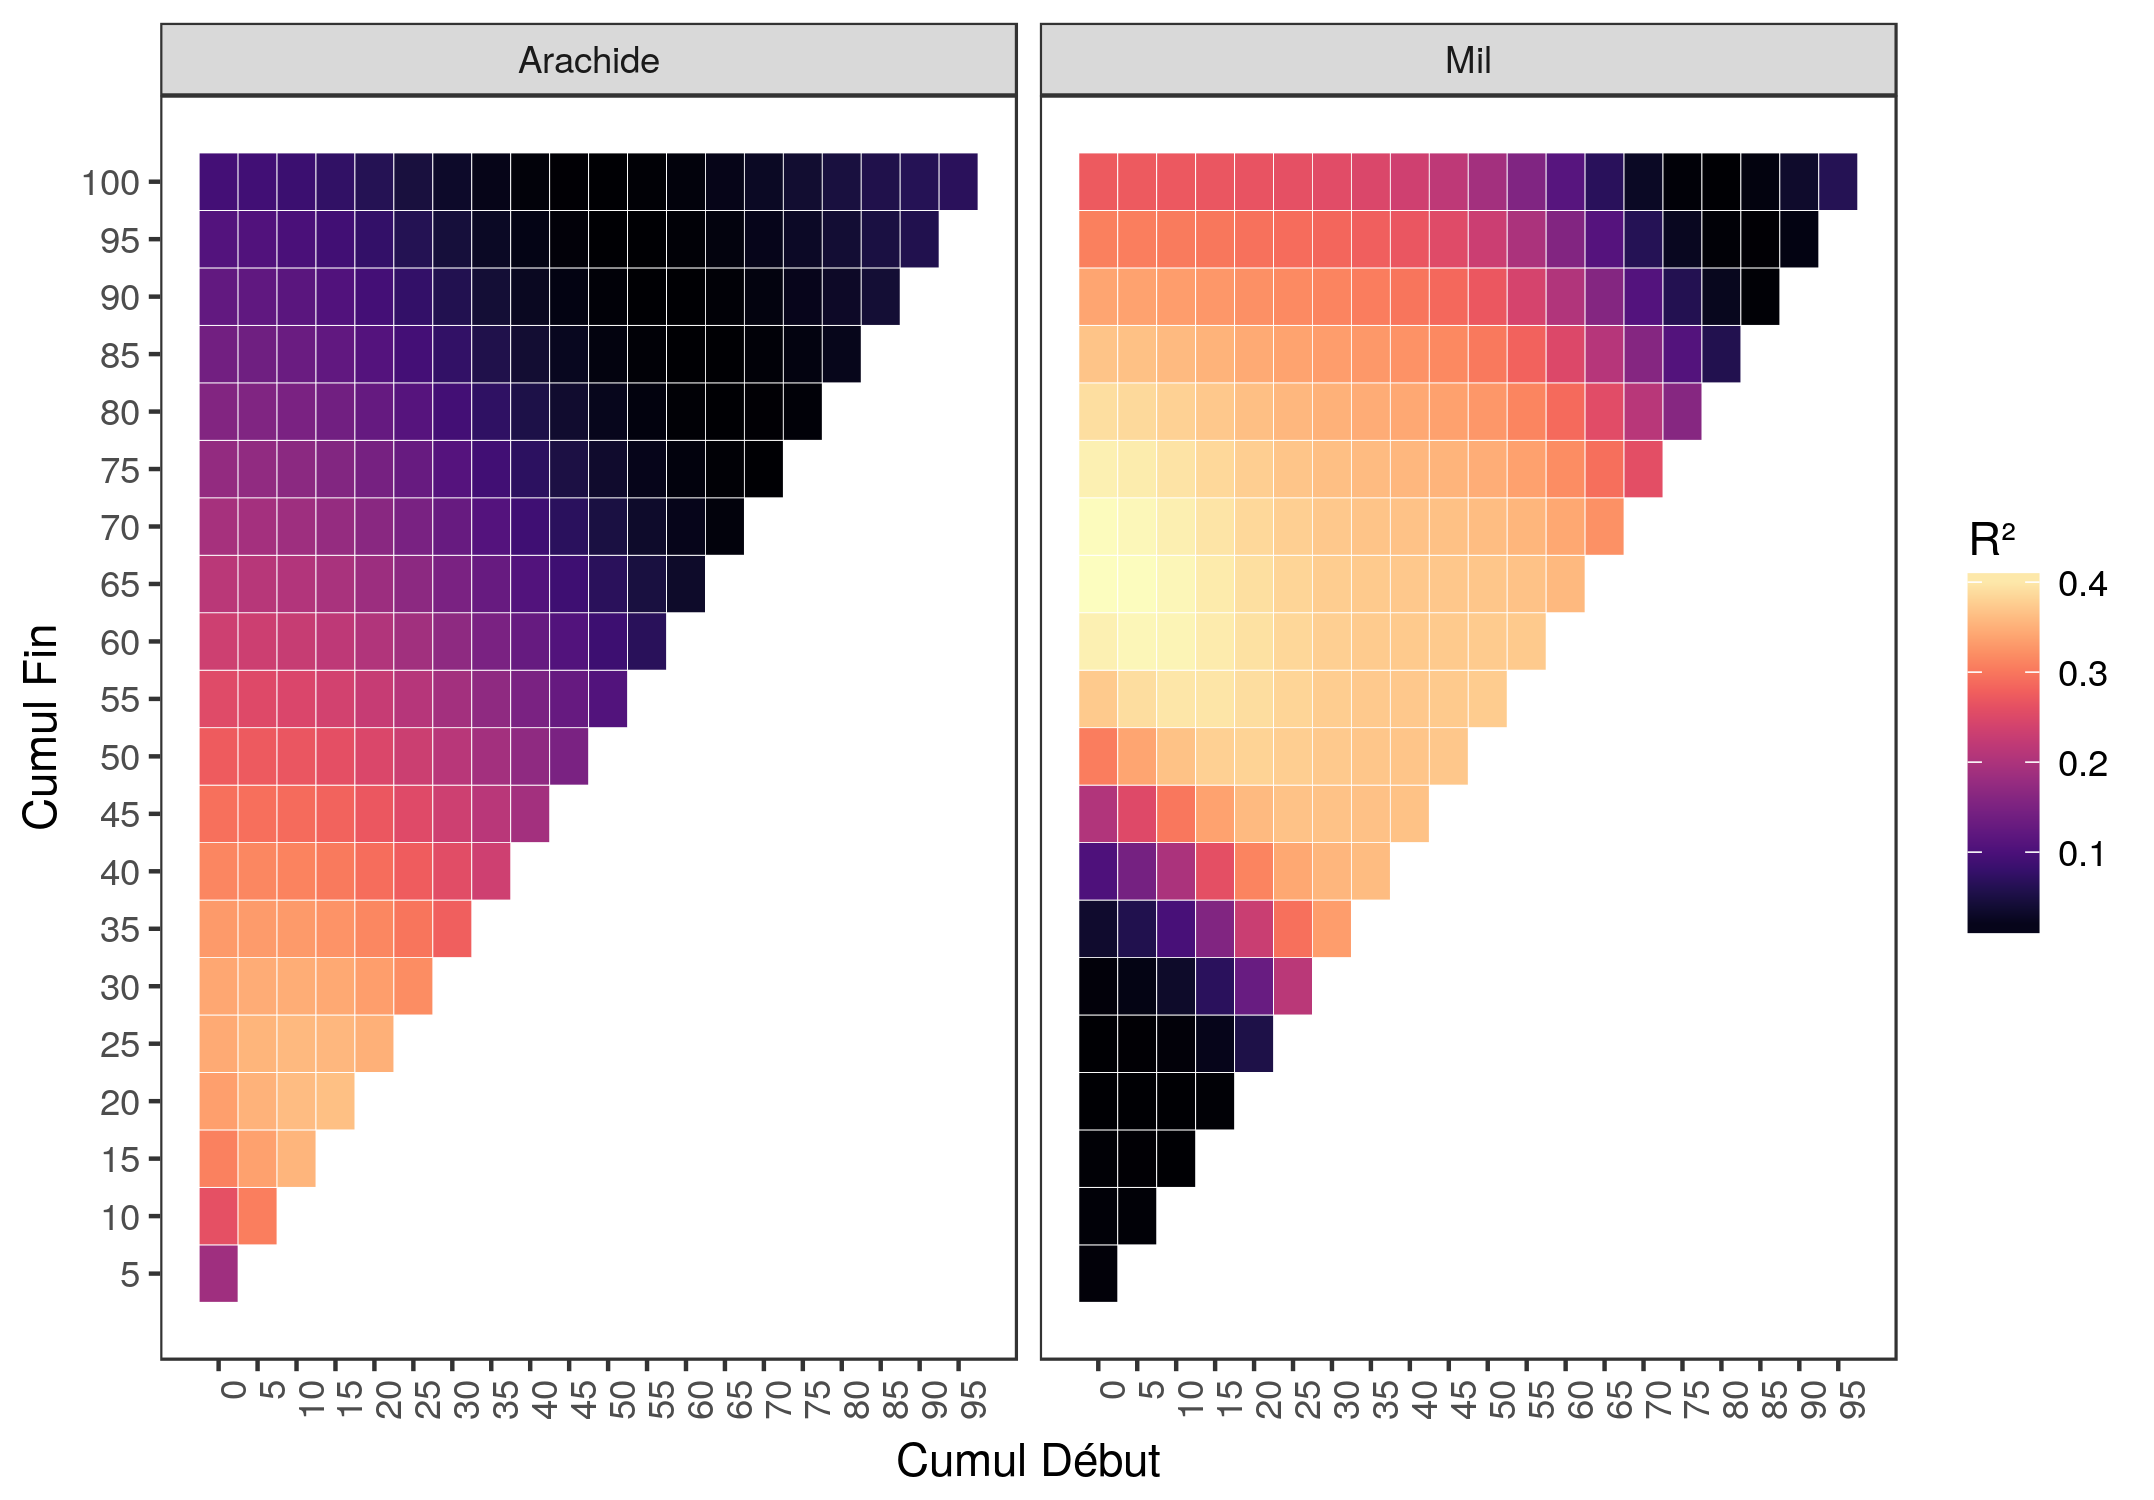
\includegraphics[scale=0.7]{resultats_discussions/Cum_Rdt_GDVI.png} 
 \end{center}
 \caption[Régressions linéaires entre cumuls de GDVI et rendements]{Résultats des régressions linéaires entre les cumuls de GDVI et les rendements}
 \label{fig-cum-rdt-gdvi}
\end{figure}

\begin{figure}[htbp]
 \begin{center}
  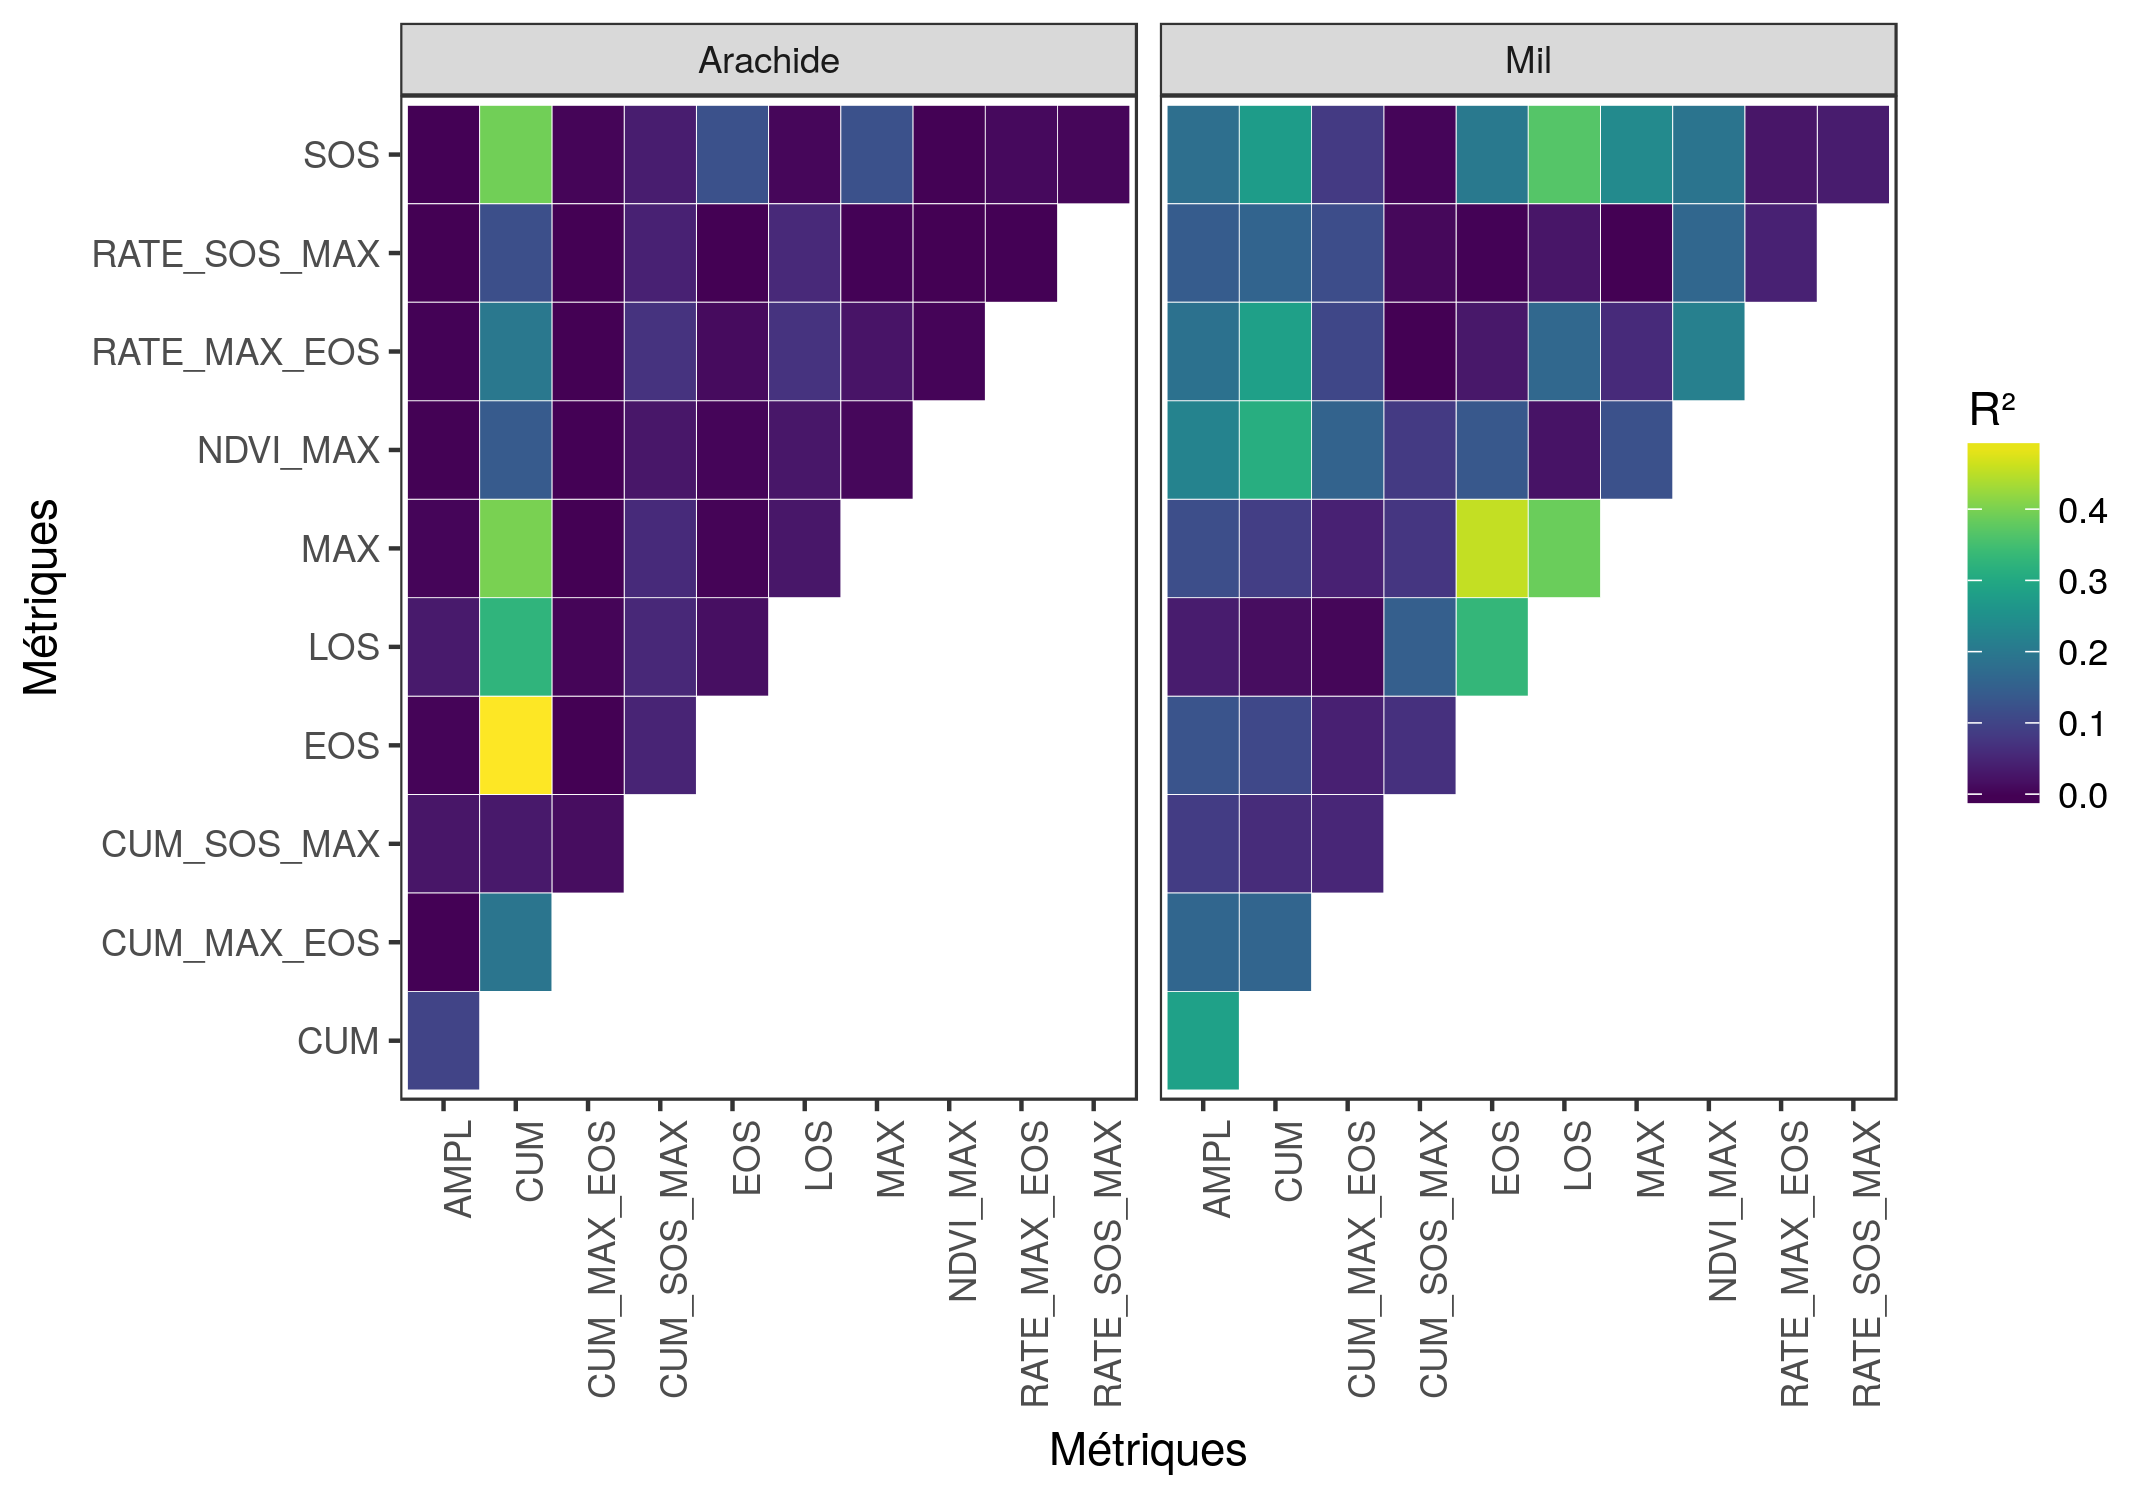
\includegraphics[scale=0.7]{resultats_discussions/Inter_Rdt.png} 
 \end{center}
 \caption[Régressions linéaires entre interactions et rendements]{Résultats des régressions linéaires entre les interactions de variables et les biomasses (\emph{l’axe des x donne le premier élément de l’interaction et l’axe des y le second ; le résultat de la régression linéaire entre l’interaction du SOS et du LOS ($SOS : LOS$) et les rendements est donné par le croisement de la lecture de SOS sur l’axe des x et LOS sur l’axe des y})}
 \label{fig-inter-rdt}
\end{figure}

\vspace{5mm}

Les résultats des régressions entre les interactions de variables et les rendements
de l’arachide et du mil sont reportés sur la \cref{fig-inter-rdt}. L’interaction entre le EOS et le $CUM_{GDVI:15-20}$ est celle qui ressort pour les rendements de l’arachide avec un $R^{2}$ de $0,497$ et une p--value de $0,01$. Pour le mil, c’est l’interaction entre le MAX et le EOS qui explique le mieux les rendements avec un $R^{2}$ de $0,453$ et une p--value de $9,36\times10^{-6}$ tout comme c’était le cas pour la biomasse. Les interactions entre variables expliquent mieux les rendements de l’arachide et du mil que les périodes d’intégration des indices seules. Au final, nous avons adopté les modèles de régression linéaire avec les interactions de variables respectivement $EOS : CUM_{GDVI:15-20}$ et $MAX : EOS$ pour l’estimation des rendements de l’arachide et du mil (\Cref{fig-model-rdt}).

\begin{figure}[htbp]
 \begin{center}
  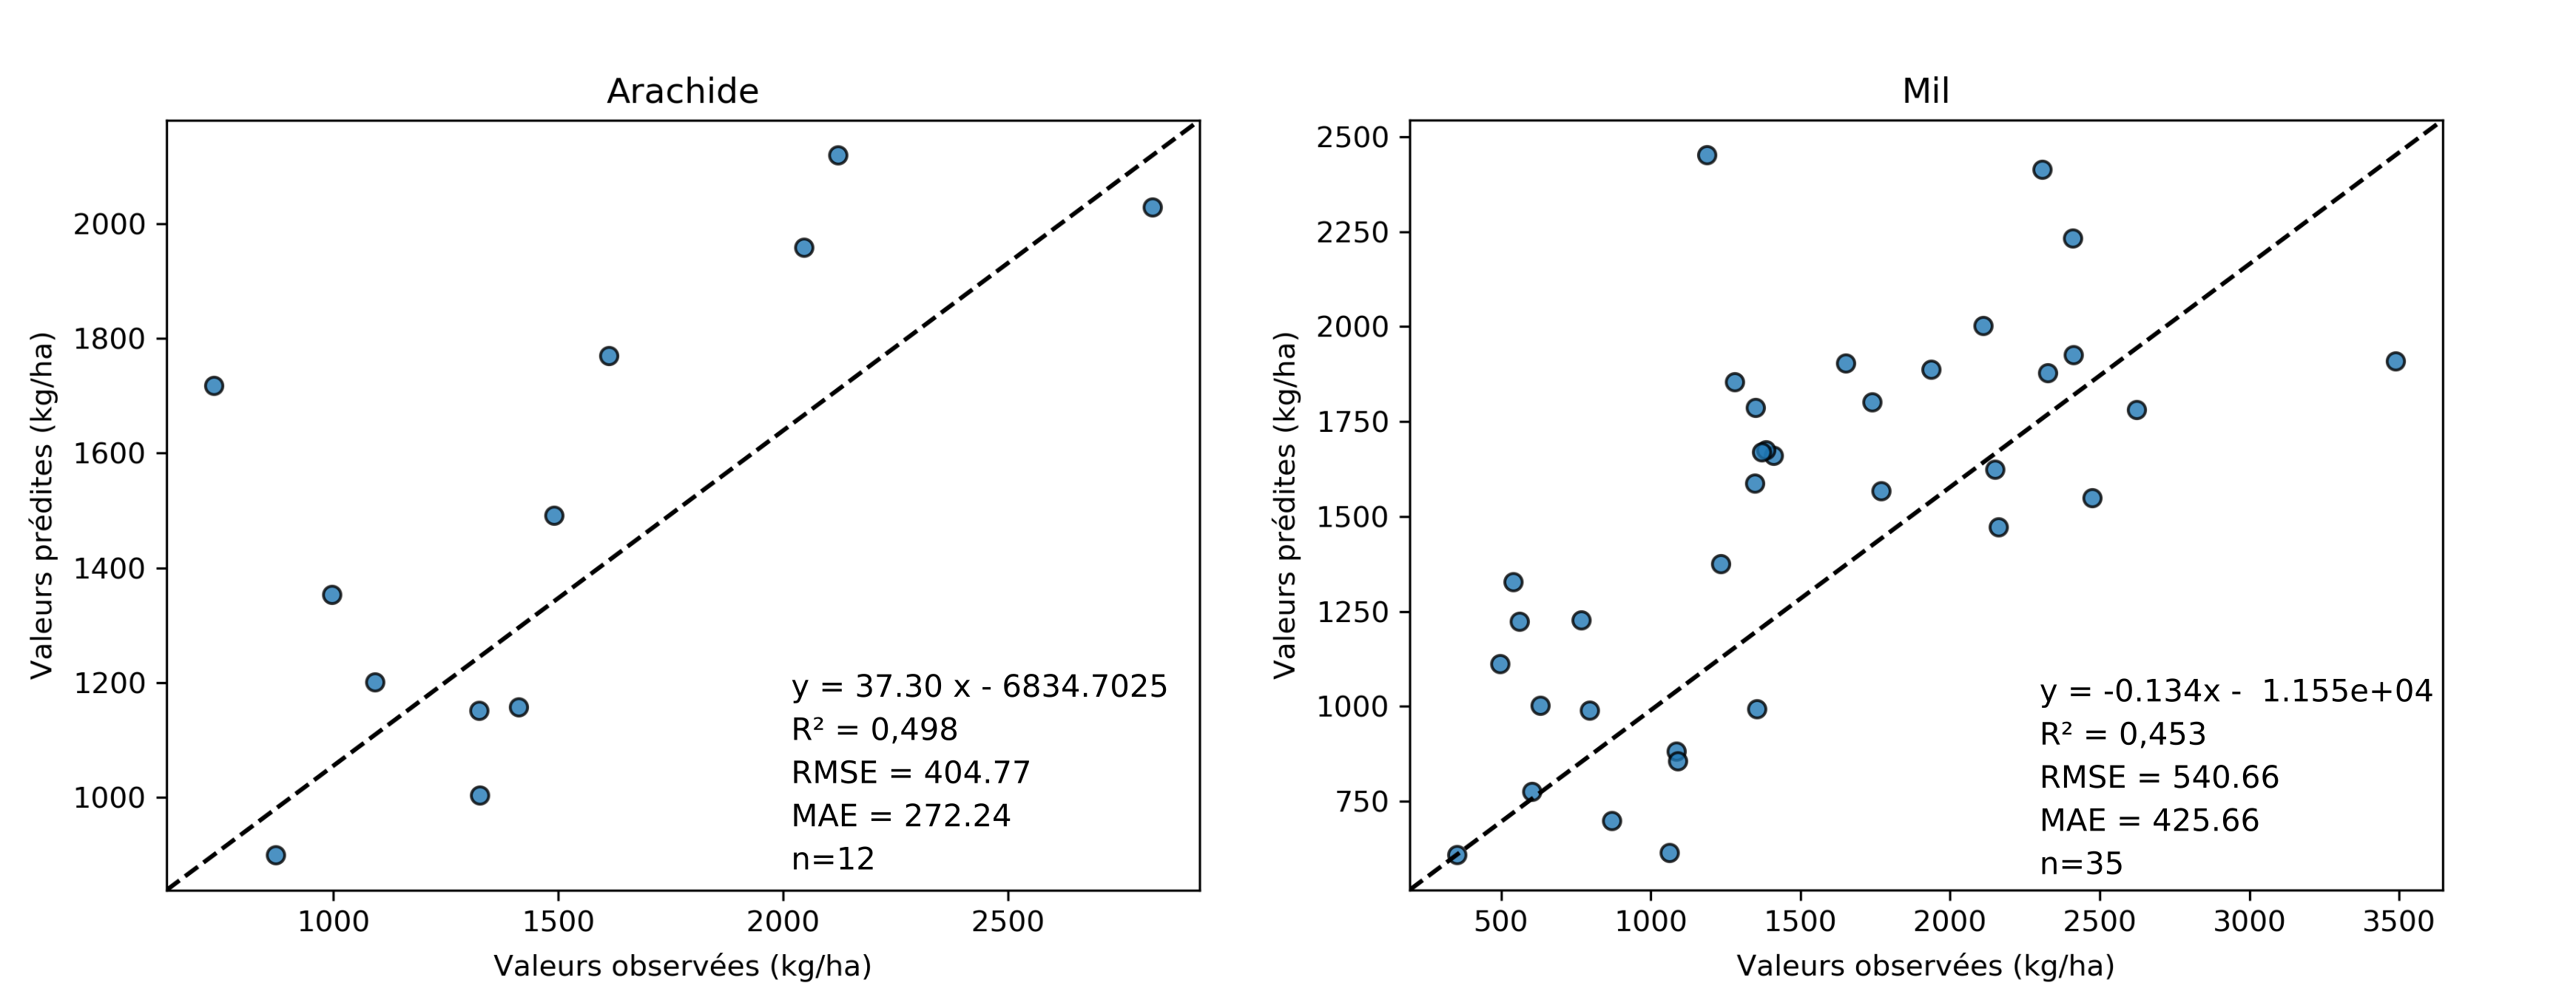
\includegraphics[scale=0.6]{resultats_discussions/Model_Rdt.png} 
 \end{center}
 \caption[Modèles finaux pour l’estimation des rendements]{Modèles finaux pour l’estimation des rendements de l’arachide et du mil}
 \label{fig-model-rdt}
\end{figure}
  
\section{Discussions}

\subsection{Sur l'extraction du SOS et du EOS}

L’approche par seuillage relatif sur les amplitudes de NDVI et le test de plusieurs seuils nous ont permis de choisir les meilleures estimations possibles des SOS et EOS. Les parcelles d’arachide ont montré les variabilités les plus faibles des écarts entre
SOS et dates de semis (plus ou moins 5 jours) suivies des parcelles de mil en culture pure (plus ou moins 10 jours) et des parcelles de mil en culture associée (plus ou moins 20 jours). Cette différence entre parcelles d’arachide et de mil tout d’abord peut s’expliquer par les pratiques culturales. En effet, les agriculteurs sèment l’arachide dès les premières pluies significatives qui arrivent à la fin Juin ou début Juillet, ce qui a tendance à harmoniser les dates de semis. Les semis du mil par contre sont plus aléatoires. Les agriculteurs sèment le mil à sec avant les premières pluies avec des semis pouvant aller jusqu’à un mois avant le démarrage effectif de la saison des pluies. Par ailleurs, si la première pluie n’est pas suffisamment efficace cela peut entraîner un échec des premiers semis et conduire à la mise en place d’un second semis. Ensuite, l’estimation des SOS est influencée par la mixité du signal capté sur les parcelles de mil en cultures associées, ce qui se traduit par une variabilité plus grande
observée sur les parcelles de mil associé. Cette même raison peut en partie expliquer la grande variabilité observée sur les écarts entre dates de EOS estimées et dates de récoltes observées, à l’exception des parcelles de mil en culture pure.
\\En ce qui concerne les seuils testés, les meilleures estimations des SOS ont été faites avec 20\% de l’amplitude du NDVI pour les parcelles d’arachide et 10\% pour les parcelles de mil. Les meilleurs EOS ont quant à eux été extraits avec 50\% les parcelles d’arachide et 80\% pour les parcelles de mil. Le seuil de 20\%, correspondant le plus
souvent au stade de déploiement des feuilles \citep{Misra2016}, est communément adopté pour les SOS \citep{Brandt2016} tandis que pour les EOS, il est plus difficile de s’accorder sur un seuil particulier tant la fin de saison peut être influencée par de nombreux facteurs (stress, ravageurs \ldots). Cependant, les différences observées entre les seuils d’extraction des EOS adoptés (50\% pour l’arachide et 80\% pour le mil) sont déterminées par les pratiques de récoltes. En effet, le mil est récolté très tôt, entre la mi-septembre et la mi-octobre selon les années en coupant uniquement les épis (les tiges et feuilles sont généralement laissées sur la parcelle et ramassées au cours de la
saison sèche) tandis que les arachides sont arrachées et récoltées plus tard en Octobre, voire début Novembre. Ainsi, en tenant compte du profil temporel de la végétation, c’est à partir de seuils élevés que les EOS extraits pourront se rapprocher des dates de récoltes du mil et à partir de seuils plus faibles que les dates de récoltes des parcelles d’arachide seront approchées.
\\Outre le test de différents seuils possibles pour la détection des dates de démarrage et de fin de saison, nous avons aussi comparé deux méthodes de lissage : HANTS et Whittaker. Nous avons montré que la méthode de lissage de Whittaker était plus à même d’estimer les dates de début de croissance de la végétation que HANTS. L’algorithme HANTS est basé sur une analyse harmonique (sommes de fonctions sinusoïdales) qui peut conduire à des fausses oscillations des profils temporels reconstruits comme cela a été le cas en début de cycle. Ces fausses oscillations produites par les méthodes basées sur la décomposition de Fourier ont été également soulignées par \citet{Hermance2007, Lu2007,Roerink2000,Jonsson2002,Chen2004}.

\subsection{Sur l'estimation des biomasses et rendements}

L’estimation des biomasses et rendements de l’arachide et du mil a révélé tout d’abord que l’utilisation du seul indice NDVI et des métriques dérivées était insuffisante pour expliquer une part satisfaisante de leurs variabilités. Si les périodes
d’intégration du NDVI sont plus nombreuses à être corrélées à la biomasse et aux rendements de l’arachide et du mil que celles du GDVI, ce sont bien les cumuls de valeurs de GDVI qui expliquent le mieux les biomasses et rendements observés. Les études menées jusqu’à présent sur l’estimation des rendements en Afrique de l’Ouest
étaient basées essentiellement sur des séries temporelles NDVI à basse résolution spatiale comme MODIS ou NOAA---AVHRR et ne prenaient pas en considération d’autres indices de végétation (ex. \citet{Leroux2016, Maselli2000,Rasmussen1997}).
Les récents travaux menés sur le continent africain avec des données à haute résolution spatiale, temporelle et spectrale mieux adaptées à l’hétérogénéité spatiale et temporelle des systèmes de culture en place ont permis de mettre en évidence des indicateurs plus performant que le NDVI pour l’estimation des rendements. Au Mali, \citet{Lambert2018} ont montré que le red edge NDVI au maximum de la saison dérivés de Sentinel-2 permettait une meilleure estimation des rendements du mil que le NDVI. Au Kenya, \citet{Jin2017} ont quant à eux montré que les prédictions des rendements du maïs à partir du MERIS Terrestrial Chlorophyll Index dérivés de RapidEye et Sentinel-2 étaient supérieures à celles faites à partir du NDVI. Les résultats de notre étude corroborent donc les tendances observées dans les récents travaux menés
dans le domaine.
\\Nos résultats ont également montré que les rendements en grain du mil étaient mieux estimés par nos modèles que la biomasse végétative. Sachant que la biomasse végétative est linéairement reliée au FAPAR (Monteith, 1972) d’une part qu’il a d’autre part était montré une relation linéaire entre le FAPAR et des indices de végétation
comme le NDVI \citep{Myneni1994}, les résultats que nous obtenons sont
surprenants. Ces résultats peuvent en partie s’expliquer par la mixité du signal reçu sur les parcelles de mil en cultures associées, où l’association avec le niébé qui est une culture couvrante à fort taux d’activité chlorophyllienne peut contribuer de façon significative au signal capté. Concernant le cas spécifique de l’arachide, nous avons
constaté globalement une meilleure capacité de nos modèles finaux de télédétection à estimer la biomasse ($R^{2} = 0,56$) que les rendements gousses ($R^{2} = 0,49$). Ces résultats s’expliquent notamment par le fait que, s’il existe une relation linéaire entre la biomasse végétative et la biomasse grain pour le cas du mil ($R^{2} = 0,78$) lorsque l’on regarde les données observées, voir \cref{annexe-e}), cette relation est plus modérée pour le cas de l’arachide entre la biomasse végétative et le rendement gousse ($R^{2} = 0,45$), voir \cref{annexe-e}). Ceci traduit donc le fait que la quantité d’activité photosynthétique produite par la plante n’est pas proportionnelle au nombre de gousses qui se développent sous terre.
\\Enfin concernant les variables explicatives les plus corrélées à la biomasse et au rendement, nous avons vu que dans le cas de l’arachide c’est l’interaction entre le GDVI cumulé sur l’ensemble du cycle de la plante ($CUM_{GDVI:15-100}$) et la date de fin (EOS) qui explique le mieux la biomasse végétative finale. Sachant qu’à la fin de la saison,
l’ensemble des biomasses végétatives pour l’arachide sont arrachées et retirées des parcelles, marquant donc un arrêt quasi-total de l’activité chlorophyllienne, cette interaction n’est pas surprenante. Pour le cas du rendement gousse, il s’agit du GDVI cumulé sur une période allant du $15^{\grave{e}me}$ au $20^{\grave{e}me}$ jour après l’émergence, correspondant au premier stade de la phase reproductive de l’arachide, soit l’ouverture des premières fleurs \citep{Boote1982}. Ce résultat est surprenant et demande plus d’investigations car à notre connaissance ce n’est pas le stade de développement le plus
déterminant pour le rendement gousse de l’arachide. Pour le mil, la variable qui explique le mieux la biomasse végétative est le GDVI cumulé sur la phase végétative ($CUM_{GDVI:0-60}$), c’est-à-dire allant de l’émergence jusqu’au LAI maximum, signifiant donc un arrêt de la production de biomasse végétative par la suite. Nos résultats sont
en ce sens cohérents avec les résultats déjà obtenus pour du mil sur le Niger par \citet{Leroux2016}. Pour l’estimation des rendements grains finaux du mil, le meilleur modèle intègre une interaction entre la date du LAI (ou NDVI) maximum et la date de fin du cycle (EOS). Là encore, les résultats sont assez cohérents avec ce que l’on connaît du cycle de développement du mil, notamment (1) la date du maximum de végétation détermine en partie la phase reproductive du mil qui inclus notamment
la floraison et le remplissage des grains, étapes déterminantes pour les rendements finaux, (2) la date de fin de la saison des cultures est déterminée par la fin de la saison des pluies, par conséquent un arrêt précoce des précipitations entraîne une réduction de la période MAX---EOS et une augmentation des risques de stress hydriques en fin de cycle de développement de la plante sur les phases reproductives et de maturation des grains.
